\appendices
\section{Supplementary Model Definitions and Main Proofs}
\AppNavLabel{app:complete_proofs}
\AppNavLabel{app:proof_summary}
Definitions and proofs supplement the model, reconstruction, and calibration analysis.

\subsection{Compatible Target Measures}
\AppNavLabel{app:deferred_constructions}

The compatible client--stratum target used for opportunity correction is
\begin{equation}
    \Lambda_s^{\mathrm{tar}}
    =
    \sum_{i:s(i)=s}\varpi_i^{\mathrm{tar}}.
    \label{eq:target_stratum_mass}
\end{equation}
For $\Lambda_s^{\mathrm{tar}}>0$,
\begin{equation}
    \nu^{\mathrm{tar}}_{i\mid s}
    =
    \frac{\varpi_i^{\mathrm{tar}}}
         {\Lambda_s^{\mathrm{tar}}},
    \qquad s(i)=s,
    \label{eq:target_conditional_atomic}
\end{equation}
and $\lambda^{\mathrm{tar}}_{k\mid s}\ge0$ is a frozen public client share
with $\sum_k\lambda^{\mathrm{tar}}_{k\mid s}=1$.  Then
\begin{equation}
 \pi^{\mathrm{tar}}_{k,s}
 =
 \begin{cases}
 \Lambda_s^{\mathrm{tar}}\lambda^{\mathrm{tar}}_{k\mid s},
 & \Lambda_s^{\mathrm{tar}}>0,\\
 0, & \Lambda_s^{\mathrm{tar}}=0,
 \end{cases}
 \label{eq:target_ks_mass}
\end{equation}
and
\begin{equation}
 \pi^{\mathrm{tar}}_{k,i}
 =
 \begin{cases}
 \pi^{\mathrm{tar}}_{k,s(i)}
 \nu^{\mathrm{tar}}_{i\mid s(i)},
 & \Lambda_{s(i)}^{\mathrm{tar}}>0,\\
 0, & \Lambda_{s(i)}^{\mathrm{tar}}=0.
 \end{cases}
 \label{eq:target_ki_mass}
\end{equation}

\subsection{Correction, Constraints, and Ideal Weights}
\AppNavLabel{app:correction_constraints}
\AppNavLabel{app:ideal_factorization}
A2's usable-update mean-ignorability display is
\begin{equation}
 \mathbb{E}\!\left[
 \left.
 \frac{U_{k,r}}{q^{\mathrm{use}}_{k,r}}
 \right|
 \mathcal{H}^{\mathrm{use}}_{k,r},
 O_e=1,k_e=k,i_e=i
 \right]
 =1.
 \label{eq:A2_use_mean_ignorability}
\end{equation}
The coordinate cap and $\ell_2$ support bound in \eqref{eq:Cr} are
\begin{equation}
\begin{aligned}
 \overline\alpha_r
 &=
 \min\!\left\{
 1,
 \max\!\left\{
 \alpha_{\max},
 \frac{1}{K_r}
 \right\}
 \right\},\\
 \overline E_r
 &=
 \min\{E_{\min},K_r\}.
\end{aligned}
 \label{eq:cap_ess}
\end{equation}
The ideal untruncated factorization of the sequential weight is
\begin{equation}
 \beta^\star_{k,r}\overline a^\star_{k,r,i}
 \propto
 R_{k,r,i}O_{k,r,i}U_{k,r}
 \frac{\zeta^{o}_{k,r,i}}
 {p^{\mathrm{obs}}_{k,r,i}q^{\mathrm{use}}_{k,r}},
 \label{eq:factorized_global_weight}
\end{equation}
where
$m^\star_{k,r}=\sum_i R_{k,r,i}O_{k,r,i}a^\star_{k,r,i}$,
$\overline a^\star_{k,r,i}=R_{k,r,i}O_{k,r,i}a^\star_{k,r,i}/m^\star_{k,r}$,
$d^\star_{k,r}=1/q^{\mathrm{use}}_{k,r}$, and
$\beta^\star_{k,r}=U_{k,r}m^\star_{k,r}d^\star_{k,r}/
\sum_j U_{j,r}m^\star_{j,r}d^\star_{j,r}$.

\subsection{Proof of Proposition~\ref{prop:risk}}
\AppNavLabel{app:proof_prop1}
\begin{restated}{Proposition}{prop:risk}
Distinct normalized laws $\boldsymbol\varpi^{\mathrm{tar}}$ and
$\widetilde{\boldsymbol\rho}^{\mathrm{arr}}$ on the same finite supported
domain admit a bounded nonnegative error profile $e_i$ with
the unequal weighted means in \eqref{eq:prop1_nonidentity}.
Equality for every bounded profile implies equal laws.
\end{restated}
\begin{proof}

Set $d_i=\varpi_i^{\mathrm{tar}}-\widetilde\rho_i^{\mathrm{arr}}$.
Both laws sum to one, so $\sum_i d_i=0$.  If they differ, the positive set
$B_+=\{i:d_i>0\}$ is nonempty and the bounded nonnegative profile
$e_i=\mathbf1\{i\in B_+\}$ gives $\sum_i d_i e_i>0$.
Conversely, equality for every profile includes each coordinate indicator,
forcing $d_i=0$ for every $i$.  A particular predictor may still have zero
risk difference.
\end{proof}

\subsection{Proof of Proposition~\ref{prop:reconstruction}}
\AppNavLabel{app:proof_prop2}
\begin{restated}{Proposition}{prop:reconstruction}
Under A1--A3, for any bounded test function $\psi(k,i)$ distinct from the
Design factor of \eqref{eq:design_factor},
the normalized estimator in \eqref{eq:hajek_phi} converges in probability
to the target moment \eqref{eq:target_phi}.
Client--stratum indicators recover $\pi^{\mathrm{tar}}_{k,s}$; compatibility
\eqref{eq:target_compatibility} makes group indicators recover $\mu_g$.
\end{restated}
\begin{proof}

The target construction gives $\sum_{i:s(i)=s}\nu^{\mathrm{tar}}_{i\mid s}=1$
on positive strata and
$\sum_k\pi^{\mathrm{tar}}_{k,i}=\Lambda^{\mathrm{tar}}_{s(i)}
\nu^{\mathrm{tar}}_{i\mid s(i)}\sum_k\lambda^{\mathrm{tar}}_{k\mid s(i)}
=\varpi_i^{\mathrm{tar}}$.  On zero-mass strata both sides are zero.
Consequently $\sum_{k,i}\pi^{\mathrm{tar}}_{k,i}=1$.

For opportunity event $e$ with mark $(k,i)$, write $p_e=p^{\mathrm{obs}}_{k,r,i}$
and $q_{k,r}=q^{\mathrm{use}}_{k,r}$.  Positivity makes both inversions legal.
An observed event implies registration.  Apply
\eqref{eq:A2_use_mean_ignorability} on that branch, then the observation
conditional expectation, in temporal order:
\begin{align}
&\mathbb E\!\left[\left.\frac{O_eU_{k,r}}{p_eq_{k,r}}
\right|k_e=k,i_e=i,\mathcal H_e^{\mathrm{obs}}\right]\nonumber\\
&\quad=\mathbb E\!\left[\left.\frac{O_e}{p_e}
\right|k_e=k,i_e=i,\mathcal H_e^{\mathrm{obs}}\right]=1.
\label{eq:app_sequential_identity}
\end{align}
This is a tower-property argument, not independence of observation and
usability.  Shared client-window usability induces dependence, handled by A3's
cluster-level weak law.
For $\chi_e$ from \eqref{eq:chi_event}, integrating the mark with law
$P_r^{\mathrm{opp}}(k,i)$ cancels its opportunity denominator:
\begin{equation}
\mathbb E[\chi_e\psi(k_e,i_e)]
=\sum_{k,i}\pi^{\mathrm{tar}}_{k,i}\psi(k,i)=\Phi^{\mathrm{tar}},
\qquad \mathbb E[\chi_e]=1.
\label{eq:app_expected_numerator_event}
\end{equation}
Let $A_R=\sum_{r<R}\sum_{e\in\mathcal O_r}\chi_e\psi(k_e,i_e)$,
$B_R=\sum_{r<R}\sum_{e\in\mathcal O_r}\chi_e$, and
$N_R=\sum_{r<R}|\mathcal O_r|$.  Under A3, $N_R\to\infty$ and
\begin{equation}
A_R/N_R\xrightarrow{p}\Phi^{\mathrm{tar}},\qquad
B_R/N_R\xrightarrow{p}1,\qquad A_R/B_R\xrightarrow{p}\Phi^{\mathrm{tar}}.
\label{eq:app_hajek_limit}
\end{equation}
The positive denominator limit justifies the ratio by continuous mapping,
even with within-window dependence.  Choosing a client--stratum indicator
recovers $\pi^{\mathrm{tar}}_{k,s}$ by conditional normalization (including
the zero-stratum convention); choosing a group indicator recovers $\mu_g$
by target compatibility.  These are ideal pooled moments, not finite-window
realizability or unbiasedness of clipped multi-step updates.
\end{proof}

\subsection{Proof of Theorem~\ref{thm:calibration}}
\AppNavLabel{app:proof_theorem1}
\begin{restated}{Theorem}{thm:calibration}
Under A4, every active window has a nonempty compact convex feasible set
$\mathcal{C}_r$, and the calibration program
$\min_{\boldsymbol\alpha\in\mathcal{C}_r}J_r(\boldsymbol\alpha)$
has a unique global minimizer $\boldsymbol\alpha_r^\star$.
\end{restated}
\begin{proof}

For $K_r\ge1$, the cap/ESS definitions give
$1/K_r\le\overline\alpha_r$ and $\overline E_r\le K_r$.
Thus $\mathbf1/K_r$ satisfies the simplex, box, and squared-norm constraints.
Their intersection is nonempty, closed, convex, and bounded, hence compact.
The objective is continuous and
\begin{equation}
\nabla^2J_r=\lambda_gM_r^\top M_r+\lambda_\beta I+\lambda_vV_r
\succeq\lambda_\beta I\succ0.
\label{eq:app_P2_hessian}
\end{equation}
The debt and staleness terms are linear.  A4 therefore gives strong convexity;
compactness gives existence and strict convexity gives uniqueness on
$\mathcal C_r$.  This certifies the mathematical minimizer, not a stored
finite-precision solution.
\end{proof}

\subsection{Proof of Proposition~\ref{prop:practical_plugin}}
\AppNavLabel{app:proof_prop3}
\AppNavLabel{app:perturbation_constants}
The Lipschitz constant in \eqref{eq:g4_beta} is
\begin{multline}
C_1
=
\frac{2K_r n_r}{B_{\min}}
\Bigl(
d_{\max}\max\{L_\pi,L_p\}+a_{\max}L_q
\Bigr),\\
L_\pi=\frac{\pi^{\mathrm{tar}}_{\max}}{\pi_{\min}^2 p_{\min}},\quad
L_p=\frac{\pi^{\mathrm{tar}}_{\max}}{\pi_{\min}p_{\min}^2},\\
L_q=\min\Bigl\{\frac{1}{q_{\min}^2},\,d_{\max}^2\Bigr\},
\label{eq:g4_c1}
\end{multline}
with $L_\pi=0$ and $L_p=1/p_{\min}^2$ under Design off. These constants bound
the implemented map's sensitivity to the opportunity, observation, and usable
margins. They are worst-case envelopes, not numerical certificates.

\begin{restated}{Proposition}{prop:practical_plugin}
Assume A1, A4, A5, and A6b.  Let the stabilized window mass obey
$\mathbf{1}^{\top}b_r^{\mathcal T}\ge B_{\min}>0$ at the true margins, and let
the ideal and the implemented reference share $\mathcal{A}_r$, $M_r$, and
$\mathcal{C}_r$.  Write $\boldsymbol\beta_r^\star$ for the same-window ideal reference,
$\widehat{\boldsymbol\beta}_r$ for the implemented clipped plug-in, and
$\boldsymbol\alpha^\star(\boldsymbol\beta)$ for the unique calibration minimizer
at the fixed state.  Then the reference, weight, and composition bounds
\eqref{eq:g4_beta}--\eqref{eq:g4_comp} hold.
Here $C_1$ and its Design-on/off constants are defined in
\eqref{eq:g4_c1}.  On the shared fixed state, the bounds hold without A6a, which is sufficient
for $\varepsilon_{\mathrm{stab},r}=0$ but not necessary when normalization
cancels distortions.  Active clipping in the
reported traces retains this term.  The worst-case envelope can be loose:
the frozen Design-on constants give $L_\pi\le2\times10^{13}$.
\end{restated}
\begin{proof}



Fix an active window $r$ and the common set $\mathcal{A}_r$.  Write
$\widehat a$ and $\widehat d$ for the implemented plug-in ratios
\eqref{eq:a_stabilized} and \eqref{eq:d_use} evaluated at the estimates, and
$a^{\mathcal T}$ and $d^{\mathcal T}$ for the same two maps evaluated at the
true margins,
\[
\begin{aligned}
a^{\mathcal T}_{k,r,i}
&=
\min\Bigl\{a_{\max},
\frac{\zeta_{k,r,i}}{\max\{p^{\mathrm{obs}}_{k,r,i},p_{\min}\}}\Bigr\},\\
d^{\mathcal T}_{k,r}
&=
\min\Bigl\{d_{\max},
\frac{1}{\max\{q^{\mathrm{use}}_{k,r},q_{\min}\}}\Bigr\},
\end{aligned}
\]
where $\zeta=\pi^{\mathrm{tar}}/\max\{\pi^{\mathrm{opp}},\pi_{\min}\}$ under Design on and
$\zeta=1$ under Design off.
The floor is the one in the implemented design factor.
Write $m^{\mathcal T}$, $b^{\mathcal T}$ and
$\boldsymbol\beta_r^{\mathcal T}$ for the corresponding masses and normalized
reference.

\emph{Step 1 (the stabilization map is Lipschitz without A6a).}  The floors
and ceilings are the only sources of non-smoothness: $x\mapsto\max\{x,c\}$ and
$x\mapsto\min\{a_{\max},x\}$ are non-expansive and $x\mapsto1/x$ is
$1/c^2$-Lipschitz on $[c,\infty)$, so $x\mapsto1/\max\{x,c\}$ is
$1/c^2$-Lipschitz on $(0,\infty)$.  With $\pi^{\mathrm{tar}}\le1$,
\begin{equation}
\begin{aligned}
 \bigl\lvert a^{\mathcal T}-\widehat a\bigr\rvert
 &\le
 L_\pi\bigl\lvert\pi^{\mathrm{opp}}-\widehat\pi^{\mathrm{opp}}\bigr\rvert\\
 &\quad
 +L_p\bigl\lvert p^{\mathrm{obs}}-\widehat p^{\mathrm{obs}}\bigr\rvert,\\
 \bigl\lvert d^{\mathcal T}-\widehat d\bigr\rvert
 &\le
 L_q\bigl\lvert q^{\mathrm{use}}-\widehat q^{\mathrm{use}}\bigr\rvert,
\end{aligned}
 \label{eq:app_plugin_lipschitz}
\end{equation}
with the constants of \eqref{eq:g4_c1}.  Under Design off the opportunity
margin does not enter the map at all, so $\zeta\equiv1$ gives $L_\pi=0$ and
$L_p=1/p_{\min}^2$.  A6b bounds the right-hand sides by
$L_\pi\varepsilon_\pi+L_p\varepsilon_p$ and $L_q\varepsilon_q$.

\emph{Step 2 (mass error).}  Each sum in \eqref{eq:m_total} has at most $n_r$
terms, so
$\lvert m_k-m^{\mathcal T}_{k}\rvert
\le n_r\max_i\lvert a_{k,r,i}-a^{\mathcal T}_{k,r,i}\rvert$, and with
$b_k=m_kd_{k,r}$,
\begin{equation}
\begin{aligned}
 \bigl\lvert b_k-b^{\mathcal T}_k\bigr\rvert
 \le{}&
 d_{\max}\,n_r\,\bigl\|a-a^{\mathcal T}\bigr\|_\infty\\
 &+a_{\max}\,n_r\,\bigl\|d-d^{\mathcal T}\bigr\|_\infty .
\end{aligned}
 \label{eq:app_plugin_mass}
\end{equation}
Only the implementation-side bounds $a\le a_{\max}$ and $d\le d_{\max}$ enter
here; the ideal ratios need not lie below the ceilings, so this step does not
need A6a either.

\emph{Step 3 (H\'ajek normalization).}  For nonnegative $x,y$ with
$\mathbf{1}^{\top}x>0$,
\[
\Bigl\|\frac{x}{\mathbf{1}^{\top}x}
-\frac{y}{\mathbf{1}^{\top}y}\Bigr\|_1
\le\frac{2\|x-y\|_1}{\mathbf{1}^{\top}x},
\]
by inserting $\pm y/\mathbf{1}^{\top}x$.  Applied with $x=b^{\mathcal T}$,
whose mass is bounded below by $B_{\min}$, and combined with Step 2,
\[
\bigl\|\widehat{\boldsymbol\beta}_r
-\boldsymbol\beta_r^{\mathcal T}\bigr\|_1
\le
\frac{2K_rn_r}{B_{\min}}
\Bigl(
d_{\max}\bigl\|a-a^{\mathcal T}\bigr\|_\infty
+a_{\max}\bigl\|d-d^{\mathcal T}\bigr\|_\infty
\Bigr).
\]

\emph{Step 4 (triangle inequality).}  By \eqref{eq:eps_stab},
$\|\widehat{\boldsymbol\beta}_r-\boldsymbol\beta_r^\star\|_1
\le\|\widehat{\boldsymbol\beta}_r-\boldsymbol\beta_r^{\mathcal T}\|_1
+\varepsilon_{\mathrm{stab},r}$, and Steps 1--3 bound the first term by
$C_1(\varepsilon_\pi+\varepsilon_p+\varepsilon_q)$ with the $C_1$ of
\eqref{eq:g4_c1}: that is \eqref{eq:g4_beta}.

\emph{Support lemma.}  Under Design on,
$a>0\iff\pi^{\mathrm{tar}}>0\iff a^\star>0$ on A5's active support; under
Design off every ratio is strictly positive there.  Hence $m^{\mathcal T}$,
$b^{\mathcal T}$, $m^\star$ and $b^\star$ share a support, which is the
shared-support clause of A5.

The calibration bound \eqref{eq:g4_alpha} is the reference
non-expansion \eqref{eq:app_reference_nonexpansive}, proved later in this supplement, on the common
convex set $\mathcal{C}_r$.  The composition bound
\eqref{eq:g4_comp} is the operator $2$-norm.
\end{proof}

The constant $C_1$ is a worst-case envelope, not a numerical certificate: at
the frozen constants its Design-on value is vacuous by many orders of
magnitude, so the informative term is $\varepsilon_{\mathrm{stab},r}$.


\subsection{Proof of Proposition~\ref{prop:group_decomposition}}
\AppNavLabel{app:proof_prop4}
\begin{restated}{Proposition}{prop:group_decomposition}
Partition the supported test units into groups $\mathcal G$, which may be the
groups of $h$ or any coarsening of them, and let $\mu^{\mathrm{eval}}_g$ and
$n_g$ be the evaluation mass and the unit count of group $g$.  Write
$\mathrm{RMSE}_g=[n_g^{-1}\sum_{i:h(i)=g}(\widehat Y_i-Y_i)^2]^{1/2}$ for the
equal-weight score of group $g$.  Then
$\mathrm{RMSE}_{\mu}^2=\sum_{g\in\mathcal G}\mu^{\mathrm{eval}}_g\,\mathrm{RMSE}_g^2$.
The identity holds for fixed predictions and fixed within-group weights.
\end{restated}
\begin{proof}


For fixed predictions, the derivative along $\sum_gd_g=0$ is
$\sum_gd_g\mathrm{RMSE}_g^2/(2\mathrm{RMSE}_{\mu})$ when
$\mathrm{RMSE}_{\mu}>0$.  A ranking reversal requires opposite signs of
$\sum_g\mu_g^{\mathrm{eval}}(\mathrm{RMSE}_{g,a}^2-\mathrm{RMSE}_{g,b}^2)$
under the two evaluation measures.

  Let $w_i=\mu^{\mathrm{eval}}_{h(i)}/n_{h(i)}$ and
$e_i^2=(\widehat Y_i-Y_i)^2$.  Substituting the definition of
$\mathrm{RMSE}_{\mu}$ and regrouping the sum by group,
\[
 \sum_{i\in\mathcal I_{\mathrm{test}}}w_ie_i^2
 =\sum_{g\in\mathcal G}\mu^{\mathrm{eval}}_g
   \Bigl(\frac1{n_g}\sum_{i:h(i)=g}e_i^2\Bigr)
 =\sum_{g\in\mathcal G}\mu^{\mathrm{eval}}_g\mathrm{RMSE}_g^2 ,
\]
which is the squared identity.  The within-group weights
$\mu^{\mathrm{eval}}_g/n_g$ do not depend on the masses of the other groups, so
$\mathrm{RMSE}_g$ is independent of $d$.  When $\mathrm{RMSE}_{\mu}>0$, differentiating
$\mathrm{RMSE}_{\mu}=(\sum_g\mu^{\mathrm{eval}}_g\mathrm{RMSE}_g^2)^{1/2}$ along a
direction with $\sum_gd_g=0$ gives the stated derivative.  Apply the identity
to both methods under both weight vectors: the sign of
$\mathrm{RMSE}_{\mu,a}^2-\mathrm{RMSE}_{\mu,b}^2$ equals the sign of
$\sum_g\mu^{\mathrm{eval}}_g(\mathrm{RMSE}_{g,a}^2-\mathrm{RMSE}_{g,b}^2)$.
The two orders differ only when the sums under
$\boldsymbol\mu^{\mathrm{eval}}$ and $\boldsymbol\mu'^{\mathrm{eval}}$
have opposite signs.


This fixed-prediction identity requires a probability evaluation measure and
within-group weights independent of other groups' masses. It applies to
$\mathrm{RMSE}_{\mu}$, not to support loss, $\Delta_{\mathrm{group}}$, or
$\Delta_{c\text{-}s}$.
\end{proof}

\subsection{Proof of the Target-Debt Accounting Bound}
\AppNavLabel{app:proof_debt_bound}
\noindent\textbf{Target-debt accounting bound (restated).}
With $\mathbf Q_0=\mathbf0$, probability vectors $\boldsymbol\mu$ and
$\boldsymbol\omega_r$, nonnegative steps $\eta_r$, and inactive windows leaving
debt unchanged, the recursion in Section~\ref{subsec:debt} implies
\eqref{eq:debt_bound} whenever $S_R>0$. Vanishing mismatch additionally requires
$\|\mathbf Q_R\|_1=o(S_R)$.
\begin{proof}

Let $D_R=\sum_{r<R}\eta_rI_r(\boldsymbol\mu-\boldsymbol\omega_r)
=S_R(\boldsymbol\mu-\overline{\boldsymbol\omega}_R)$.
Projection onto the nonnegative orthant gives, coordinatewise,
\begin{equation}
Q_{r+1,g}\ge Q_{r,g}+\eta_rI_r(\mu_g-\omega_{r,g}),
\qquad (D_{R,g})_+\le Q_{R,g}.
\label{eq:app_Q_dominates_D}
\end{equation}
The second inequality follows by telescoping from $Q_{0,g}=0$;
inactive windows contribute zero and leave debt unchanged.
Both target and active-window composition have unit mass, so
$\mathbf1^\top D_R=0$.  Equal positive and negative mass then gives
\begin{equation}
S_R\|\overline{\boldsymbol\omega}_R-\boldsymbol\mu\|_1
=\|D_R\|_1=2\|(D_R)_+\|_1\le2\|\mathbf Q_R\|_1.
\label{eq:app_debt_bound_final}
\end{equation}
Divide by $S_R>0$ to obtain \eqref{eq:debt_bound}.  Vanishing mismatch follows
if $\|\mathbf Q_R\|_1=o(S_R)$; the recursion alone does not prove that
growth condition.
\end{proof}

\subsection{Supplementary Consequences of the Calibration Geometry}
\AppNavLabel{app:supp_calibration_geometry}

The following properties describe the finite-window geometry of the feasible
set and objective defined in Section~V.

\paragraph{Feasible target image}
For an active window, define the set of deployment-group compositions that can
be realized by the currently available clients as
\begin{equation}
 \Omega_r
 \triangleq
 \left\{
 M_r\boldsymbol\alpha:
 \boldsymbol\alpha\in\mathcal C_r
 \right\}.
 \label{eq:app_feasible_target_image}
\end{equation}
Under A4, $\mathcal C_r$ is nonempty, compact, and convex.  Since
$\boldsymbol\alpha\mapsto M_r\boldsymbol\alpha$ is linear, $\Omega_r$ is also
nonempty, compact, and convex.  Hence, the irreducible instantaneous
feasibility gap
\begin{equation}
 d_r^{\mathrm{feas}}
 \triangleq
 \min_{\boldsymbol\omega\in\Omega_r}
 \left\|
 \boldsymbol\omega-\boldsymbol\mu
 \right\|_2
 \label{eq:app_feasibility_gap}
\end{equation}
is attained, and
\begin{equation}
 d_r^{\mathrm{feas}}=0
 \quad\Longleftrightarrow\quad
 \boldsymbol\mu\in\Omega_r.
 \label{eq:app_exact_realizability}
\end{equation}
Thus, if $d_r^{\mathrm{feas}}>0$, no admissible aggregation rule with the same
finite-window support and constraints can exactly realize
$\boldsymbol\mu$ in that window.  Calibration should therefore be interpreted as
calibrating within the realizable image rather than synthesizing unavailable
target support.\hfill$\square$

\paragraph{Reference stability of calibration}
Fix one active window, including $M_r$, $\mathbf Q_r$, $V_r$,
$\overline{\boldsymbol\tau}_r$, $\mathcal C_r$, and all regularization
coefficients.  Let $\boldsymbol\alpha^\star(\boldsymbol\beta)$ denote the
unique calibration minimizer when the corrected reference is
$\boldsymbol\beta$.  Then, for any two reference vectors
$\boldsymbol\beta$ and $\boldsymbol\beta'$ on the same feasible support,
\begin{equation}
 \left\|
 \boldsymbol\alpha^\star(\boldsymbol\beta)
 -
 \boldsymbol\alpha^\star(\boldsymbol\beta')
 \right\|_2
 \le
 \left\|
 \boldsymbol\beta-\boldsymbol\beta'
 \right\|_2.
 \label{eq:app_reference_nonexpansive}
\end{equation}
To see this, write the calibration objective as
\begin{equation}
 G_r(\boldsymbol\alpha)
 +\frac{\lambda_\beta}{2}
 \left\|
 \boldsymbol\alpha-\boldsymbol\beta
 \right\|_2^2,
 \label{eq:app_p2_split}
\end{equation}
where $G_r$ contains the debt, group, variance, and staleness terms and is
convex under A4.  Let
$\mathbf x=\boldsymbol\alpha^\star(\boldsymbol\beta)$ and
$\mathbf y=\boldsymbol\alpha^\star(\boldsymbol\beta')$.  Adding the two
variational inequalities on the common convex set $\mathcal C_r$ gives
\begin{align}
 &\left\langle
 \nabla G_r(\mathbf x)-\nabla G_r(\mathbf y),
 \mathbf x-\mathbf y
 \right\rangle
 +\lambda_\beta\|\mathbf x-\mathbf y\|_2^2
 \nonumber\\
 &\qquad\le
 \lambda_\beta
 \left\langle
 \boldsymbol\beta-\boldsymbol\beta',
 \mathbf x-\mathbf y
 \right\rangle.
 \label{eq:app_reference_vi}
\end{align}
The first term on the left is nonnegative by monotonicity of the gradient of a
convex function.  Cauchy--Schwarz therefore yields
\eqref{eq:app_reference_nonexpansive}.
\qed

Reconstruction concerns pooled population moments; reference stability fixes
the entire window state. Neither supplies unconditional long-run alignment or
a prediction guarantee.

\section{Aggregate Coverage Diagnostic and Its Proofs}
\AppNavLabel{app:agg_coverage_proofs}
Definitions and proofs supplement the aggregate coverage diagnostic.

\subsection{Target-Positive Coverage and Lookup}
\AppNavLabel{app:itar_lookup}
$I_{\mathrm{tar}}=\{(k,s):\pi^{\mathrm{tar}}_{k,s}>0\}$ and $C_t$ in
\eqref{eq:agg_Ct} use $\pi^{\mathrm{tar}}_{k,s}$ from \eqref{eq:target_ks_mass}.
For unit $i$, $k(i)$ is the unique client on the frozen occupancy map
(stations on SensorScope and U-Air, occupied cells on T-Drive and City
Scanner). The lookup is $\pi^{\mathrm{tar}}(k(i),s(i))$; a missing key is $0$,
including when several clients meet the same unit. Table~\ref{tab:scd_phi_freeze}
is the train-unit fraction of those zeros. It is not
$\#\{i:\varpi_i^{\mathrm{tar}}=0\}$ and not a target-positive-pair check. It
enters \eqref{eq:design_gate}, and can set \eqref{eq:design_factor} only when
its inputs exist before the window; both fixed settings are reported.
$\pi^{\mathrm{opp}}_{k,s,t}$ is $F_{t-}$-measurable on the same key. Since
$\sum_{k,s}\pi^{\mathrm{tar}}_{k,s}=1$, \eqref{eq:agg_Ct} is certified mass over
positive target mass.

\subsection{Historical Quantiles and Diagnostic States}
\AppNavLabel{app:coverage_algorithm}
\begin{algorithm}[t]
\caption{Aggregate coverage certificate (diagnostic Gate)}
\label{alg:agg_certificate}
\begin{algorithmic}[1]
\REQUIRE legal $F_{t-}$; public $a_t$; block snapshot $f_b$; same-block scores;
previous CERTIFIED miscoverage flag; $\alpha=0.05$; $\tau_{\mathrm{cov}}=0.05$; $n_{\min}=19$
\ENSURE $\mathrm{state}\in\{\mathrm{WARMUP},\mathrm{CERTIFIED},\mathrm{RESET}\}$,
block\_id, predictor\_snapshot\_id, $\widehat C_t$, $n$, $q_t$ if CERTIFIED,
$C^{\mathrm{LCB}}_t$, $\mathrm{Gate}_t$
\IF{the previous completed CERTIFIED window satisfied $C^{\mathrm{LCB}}>C$}
\STATE $\mathrm{state}\leftarrow\mathrm{RESET}$, $\mathrm{Gate}_t\leftarrow\mathrm{OFF}$
\STATE Fit $f_{b+1}$ on completed past data only; freeze it; clear the buffer
\STATE $\mathrm{state}\leftarrow\mathrm{WARMUP}$
\ELSE
\STATE Use the frozen snapshot $f_b$ of the current block
\IF{$n<19$ or $k_n>n$}
\STATE $\mathrm{state}\leftarrow\mathrm{WARMUP}$
\STATE $C^{\mathrm{LCB}}_t\leftarrow 0$, $\mathrm{Gate}_t\leftarrow\mathrm{OFF}$
\ELSE
\STATE $\mathrm{state}\leftarrow\mathrm{CERTIFIED}$ \COMMENT{regime for Assumption~1}
\STATE $\widehat C_t\leftarrow f_b(F_{t-})$
\STATE $q_t\leftarrow S_{(k_n)}^{\mathrm{cal}}$ \COMMENT{no clipping of $k_n$ to $n$}
\STATE $C^{\mathrm{LCB}}_t\leftarrow\max\{0,\widehat C_t-q_t\}$
\STATE $\mathrm{Gate}_t\leftarrow \mathbf{1}\{C^{\mathrm{LCB}}_t\ge\tau_{\mathrm{cov}}\}$
\ENDIF
\ENDIF
\end{algorithmic}
\end{algorithm}

\subsection{Pairwise Opportunity Barriers}
\begin{proposition}[Positive pairwise LCB barrier]
\label{prop:pairwise-lcb-barrier}
Let $X_t\ge 0$ denote the realized opportunity of one target pair in window
$t$, and let $L_t=L(F_{t-})$ be a deterministic pre-window lower bound.  If
$P(X_t=0\mid F_{t-})>\alpha$, then no strictly positive $L_t>0$ can satisfy
$P(L_t\le X_t\mid F_{t-})\ge 1-\alpha$.
\end{proposition}

\begin{corollary}[Availability-induced pairwise barrier]
\label{cor:availability-barrier}
For a target pair $i=(k,s)$ let the designated stressed entity be $e(i)=k$
(the pair's client).  Let $A_{e(i),t}\in\{0,1\}$ be that entity's availability
in window $t$.  Assume $X_{i,t}>0\Rightarrow A_{e(i),t}=1$.  Under frozen
availability stress, $P(A_{e(i),t}=1\mid F_{t-},a)\le a$, hence
$P(X_{i,t}>0\mid F_{t-},a)\le a$.  If $a<1-\alpha$, no strictly positive
deterministic $1-\alpha$ pairwise LCB is guaranteed for that pair under
Proposition~\ref{prop:pairwise-lcb-barrier}.  The claim applies only to pairs
obeying the designated-entity necessary condition.
\end{corollary}

\subsubsection{Proof of Proposition~\ref{prop:pairwise-lcb-barrier}}
\AppNavLabel{app:proof_pairwise_lcb}
\begin{proof}
Fix a regular conditional probability given $F_{t-}$. On $\{L_t>0\}$,
$\{L_t\le X_t\}\subseteq\{X_t>0\}$, because $X_t=0$ makes the bound fail.
Consequently,
\[
P(L_t\le X_t\mid F_{t-})\le1-P(X_t=0\mid F_{t-})<1-\alpha.
\]
Hence a deterministic nonnegative bound satisfying the claimed coverage must
be zero wherever the stated zero-opportunity condition holds.
\end{proof}

\subsubsection{Proof of Corollary~\ref{cor:availability-barrier}}
\AppNavLabel{app:proof_availability_barrier}
\begin{proof}
The necessary condition $X_{i,t}>0\Rightarrow A_{e(i),t}=1$ gives
\[
P(X_{i,t}>0\mid F_{t-},a)
\le P(A_{e(i),t}=1\mid F_{t-},a)\le a.
\]
Thus $P(X_{i,t}=0\mid F_{t-},a)\ge1-a>\alpha$ when $a<1-\alpha$.
Proposition~\ref{prop:pairwise-lcb-barrier} then excludes a strictly positive
pairwise LCB. The conclusion requires the designated-entity condition.
\end{proof}

\subsection{\texorpdfstring{$n_{\min}$}{n-min} derivation}
\AppNavLabel{app:nmin}

A finite historical quantile requires
$k_n=\lceil(n+1)(1-\alpha)\rceil\le n$, equivalently
$n\ge\lceil1/\alpha\rceil-1$. Thus $\alpha=0.05$ gives $n_{\min}=19$.
Below this size, the required order statistic is $n+1$, corresponding to
$q=+\infty$. Replacing it with the sample maximum does not restore nominal
coverage; in particular, $n=8$ is insufficient for a finite 95\% bound.

\subsection{Proof of Theorem~\ref{thm:agg-lcb}}
\AppNavLabel{app:proof_agg_lcb}
\begin{restated}{Theorem}{thm:agg-lcb}
Assume window $t$ is in operational state CERTIFIED, $n\ge n_{\min}=19$,
Assumption~\ref{ass:score-exchangeability} holds, $\widehat C_t=f_b(F_{t-})$
uses the frozen predictor snapshot of the current block, and the calibration
scores are strictly historical same-block scores.  Let
$q_t=S_{(k_n)}^{\mathrm{cal}}$ with $k_n$ from \eqref{eq:agg_kn}, and define
$C^{\mathrm{LCB}}_t$ by \eqref{eq:agg_CLCB}.  Then the lower-coverage bound \eqref{eq:agg_thm1} holds.
CERTIFIED is an operational state, not evidence for exchangeability.
\end{restated}
\begin{proof}
Conditionally on $g$, attach independent continuous tie-breaks to the $n$
historical scores and $S_t$. Exchangeability makes the rank $R_t^\star$ of
the current score uniform on $\{1,\ldots,n+1\}$. CERTIFIED ensures
$k_n\le n$, so $q_t$ is a finite calibration order statistic and
\[
P(R_t^\star\le k_n\mid g)=k_n/(n+1)\ge1-\alpha.
\]
If $S_t>q_t$, at least $k_n$ historical scores are strictly smaller, forcing
$R_t^\star\ge k_n+1$. Thus
$\{R_t^\star\le k_n\}\subseteq\{S_t\le q_t\}$.
Since $S_t=\widehat C_t-C_t$ and $C_t\ge0$, this event implies
$\max\{0,\widehat C_t-q_t\}\le C_t$, giving
\[
P(C_t^{\mathrm{LCB}}\le C_t\mid g)
\ge P(S_t\le q_t\mid g)\ge1-\alpha.
\]
The current outcome enters the calibration buffer only after completion;
exchangeability remains an assumption.
\end{proof}

\subsection{Proof of Corollary~\ref{cor:false-safe-gate}}
\AppNavLabel{app:proof_false_safe}
\begin{corollary}[False-safe Gate bound]
\label{cor:false-safe-gate}
Under the conditions of Theorem~2,
\begin{equation}
 P\bigl(\mathrm{Gate}_t=1\text{ and }C_t<\tau_{\mathrm{cov}}\mid g\bigr)
 \le\alpha.
 \label{eq:agg_cor2}
\end{equation}
\end{corollary}

\begin{proof}
On the event $\{\mathrm{Gate}_t=1,\,C_t<\tau_{\mathrm{cov}}\}$ one has
$C^{\mathrm{LCB}}_t\ge\tau_{\mathrm{cov}}>C_t$, hence
$C^{\mathrm{LCB}}_t>C_t$.  Therefore
\[
 \{\mathrm{Gate}_t=1,\,C_t<\tau_{\mathrm{cov}}\}
 \subseteq
 \{C^{\mathrm{LCB}}_t>C_t\}.
\]
Theorem~2 gives $P(C^{\mathrm{LCB}}_t\le C_t\mid g)\ge 1-\alpha$,
so $P(C^{\mathrm{LCB}}_t>C_t\mid g)\le\alpha$.  The false-safe probability is
at most $\alpha$.  In WARMUP and RESET, $\mathrm{Gate}_t$ is OFF by definition,
so the false-safe event is empty on those windows.
\end{proof}

\subsection{Proof of Proposition~\ref{prop:drift-boundary}}
\AppNavLabel{app:proof_drift_boundary}
\begin{proposition}[Arbitrary-drift applicability boundary]
\label{prop:drift-boundary}
Suppose two data-generating worlds share the same legal $F_{t-}$ but have
$C_t=c_{\mathrm{high}}$ and $C_t=c_{\mathrm{low}}$ with
$c_{\mathrm{low}}<\tau_{\mathrm{cov}}<c_{\mathrm{high}}$.  Any deterministic
pre-window certificate outputs the same $C^{\mathrm{LCB}}_t$ in both worlds.
If that output is at least $\tau_{\mathrm{cov}}$, the certificate is
false-safe in the low world; if it is below $\tau_{\mathrm{cov}}$, it cannot
certify the high world.  Without an assumption linking the current window to
observable pre-window information, no method can simultaneously provide
nontrivial per-window certification and universal protection against
arbitrary unannounced regime shifts.
\end{proposition}

\begin{proof}
The two worlds share $F_{t-}$, hence the pre-window rule has the same output
$L$ in both. If $L\ge\tau_{\mathrm{cov}}$, it exceeds $c_{\mathrm{low}}$
and is false-safe in the low-coverage world. Otherwise it cannot certify the
high-coverage world, where $c_{\mathrm{high}}>\tau_{\mathrm{cov}}$.
Independent auxiliary random bits do not distinguish the worlds either.
After detection, RESET/WARMUP keeps Gate off until the new regime has enough
history; it does not restore Theorem~\ref{thm:agg-lcb} on an undetected first-shift window.
\end{proof}

\section{Experimental Protocols and Baseline Specifications}
\AppNavLabel{app:experimental_protocols}
Protocols and baseline definitions complement the evaluation settings.

\subsection{City Scanner New York \texorpdfstring{{PM}$_{2.5}$}{PM2.5}}
\AppNavLabel{app:cityscanner_nyc}

New York Pilot~1/2 {PM} CSVs (Zenodo 10.5281/zenodo.7961851, {CC BY}
4.0)~\cite{wang2023cityscanner} exclude Boston, Beirut, and {NO}$_2$.
Non-finite GPS, time, or {PM}$_{2.5}$, and values outside
$[0,1000]$\,$\mu$g/m$^3$, are removed. Occupied $500$\,m $\times$ $30$\,min
cells average calibrated measurements into $Y$; empty slots are absent.
Cells are clients and GPS supplies $R$. Median cell indices define four
quadrants without $Y$; $\boldsymbol\mu$ is their test share. Strata are
$\mathrm{region}{::}\mathrm{block}{::}\mathrm{weekday}$ (at most 32).
Complete-aligned $O/U$ use $p_{\mathrm{obs}}=.35$ and $S_{\max}=5$.

The 14723 units, 446 cells, and 2776 slots split chronologically into
$9343/3290/2090$ train/validation/test units (test regions $496/992/148/454$).
Seeds $32001$--$32010$ share 100 equal-count windows of 1666 training slots.
Design is on and Gate is unused (Table~\ref{tab:scd_phi_freeze}).
Table~\ref{tab:cityscanner_real}(a) uses training-standardized errors. One
seed-32006 window clipped and renormalized tiny negative solver weights.

\subsection{City Scanner Pilot~2 with Measured Observation}
\AppNavLabel{app:cityscanner_p2_measured_o}

Pilot~2 uses {PM}/{NO}$_2$ CSVs from the same source, excluding Pilot~1,
Boston, and Beirut, on the same client/$Y$ grid. Union GPS supplies $R$;
finite {PM}$_{2.5}$ in $[0,1000]$ supplies $O=1$; {NO}$_2$ contributes
locations only. $U$ stays Complete-aligned ($S_{\max}=5$). The frozen regional
target, Design-on, and unused Gate keep their roles at different target values.

The 14960 cell-slots, 416 cells, and 2402 slots split into
$10141/2835/1984$ train/validation/test units: 1931 unobserved ($12.9\%$) and
13029 labeled, with test-region occupancy $1289/268/144/283$. Seeds
$33001$--$33010$ use 100 windows from 1441 training slots.
Table~\ref{tab:cityscanner_real}(b) uses this block's training standardization.
Section~\ref{subsec:cityscanner_real} gives the rankings and the missed
improvement criterion.

\subsection{Windowed adaptations of FedAU, ObsUse, and TimeAlign}
\AppNavLabel{app:adapted_baselines}
FedAU~\cite{wang2024lightweight} targets the original federated averaging
objective under unknown participation; these rules reweight usable clients
and do not recover that objective.
After window close, each EventTrace record of client \(k\) increments
\(N^{\mathrm{att}}_k\), and \(N^{\mathrm{use}}_k\) if it is a registered
usable update.  Window \(r\) uses earlier windows
(\(\varepsilon=10^{-6}\); unseen rate \(1\)).
Let \(n_{k,r}\) be the observed-unit count (empty buffer encoded as one),
\(\widehat p^{\mathrm{obs}}_{k,r}\) the mean frozen observation propensity
on the current risk set clipped below at \(0.05\) (or \(1\) if empty),
\(S_k\) the covered slots on \(\mathcal{A}_r\), and
\(\mathrm{overlap}(s)=\#\{j\in\mathcal{A}_r:s\in S_j\}\).
\begin{align}
 \widehat p^{\mathrm{part}}_{k,r}
 &=
 (N^{\mathrm{use}}_k+\varepsilon)/(N^{\mathrm{att}}_k+\varepsilon),
 \label{eq:fedau_part_rate}\\
 \alpha^{\mathrm{FedAU}}_{k,r}
 &\propto n_{k,r}/\max\{\widehat p^{\mathrm{part}}_{k,r},\varepsilon\},
 \label{eq:fedau_window_alpha}\\
 \alpha^{\mathrm{ObsUse}}_{k,r}
 &\propto n_{k,r}/(\widehat p^{\mathrm{obs}}_{k,r}\widehat p^{\mathrm{part}}_{k,r}),
 \label{eq:obsuse_window_alpha}\\
 \alpha^{\mathrm{TimeAlign}}_{k,r}
 &\propto \sum_{s\in S_k}1/\mathrm{overlap}(s).
 \label{eq:timealign_window_alpha}
\end{align}
FedAU-Window uses \eqref{eq:fedau_window_alpha} only.
ObsUse-Window uses \eqref{eq:obsuse_window_alpha} and omits Design, calibration, and debt.
TimeAlign-Agg (\texttt{flamf\_timealign\_adapted}) uses
\eqref{eq:timealign_window_alpha} following~\cite{wang2026federated},
with overlap-based weights and the shared window-close protocol.
Paired methods share the Common-NDMF backbone, step size, and selection
trace (seeds \(30001\)--\(30020\)).  Existing tables already report
these adaptations.



\begin{table*}[t]
\begin{minipage}{\textwidth}
\normalsize
\subsection{Selection Mechanisms and Information Requirements}
\AppNavLabel{app:mechanism_comparison}
Table~\ref{tab:nearest_neighbor} compares the selection units, available
information, target objects, and guarantee scopes of FedIPW, FedPALS,
and RAVEN-MCS.
\end{minipage}
\smallskip

\centering
\caption{Selection mechanisms and their information requirements.}
\label{tab:nearest_neighbor}
\footnotesize
\setlength{\tabcolsep}{3pt}
\begin{tabular}{@{}p{1.8cm}p{4.2cm}p{4.2cm}p{6.0cm}@{}}
\toprule
Dimension & FedIPW~\cite{morishita2026who} & FedPALS~\cite{listozec2024overcoming} & RAVEN-MCS\\
\midrule
Selection unit & Client enrollment and round participation & Client/source label distribution & Atomic sensing opportunity/observation, then registered update usability\\
Available information & Pre-enrollment/pre-round covariates; population summaries in calibration extension & Known client and target label marginals, client sample sizes & Public atomic/group target; lagged opportunity, pre-$O$ covariates, pre-$U$ registration history\\
Target object & Target-population mean update & Target-domain risk under label shift & Deployment measure over sensing units and compatible client--stratum mass\\
Correction / reference & Product IPW; enrolled-sample calibration & Convex composition matching & Sequential normalized correction forms $\widehat\beta_r$ before feasible calibration\\
Caps / ESS & Population-summary constraints; no corresponding window caps/ESS & Soft inverse sample-level ESS penalty & Hard client cap and client-level ESS ball on current $\mathcal A_r$\\
Cross-window state & Propensity estimation & Recomputed target-aware weights & Lagged selection/variance histories and target debt\\
Guarantee scope & Mean-update identification; residual-weight analysis under stated optimization assumptions & One-step unbiased update under label shift and convex-hull coverage & Ideal pooled moments; fixed-state calibration stability; conditional debt accounting\\
\bottomrule
\end{tabular}
\end{table*}
\FloatBarrier

\section{Additional Results for Deployment-Target Alignment}
\AppNavLabel{app:rq1_results}

\AppNavLabel{app:risk_semantic_evidence}
These supplementary results address deployment alignment in RQ1.

\subsection{Full Method Context on the Comparable Datasets}
\AppNavLabel{app:e3_full_context}

\begin{table}[!htbp]
\centering
\caption{SensorScope method comparison.
Mean $\pm$ SD over 20 seeds; lower is better.
$^\dagger$ denotes reference-only context.}
\label{tab:app_e3_sensorscope}
\footnotesize
\setlength{\tabcolsep}{1.5pt}
\begin{tabular*}{\columnwidth}{@{\extracolsep{\fill}}lccc}
\toprule
Method & $\mathrm{RMSE}_{\mu}$ & $\Delta_{\mathrm{group}}$ & $\Delta_{c\text{-}s}$\\
\midrule
Central-All$^{\dagger}$ & $7.6004\pm0.0695$ & -- & -- \\
Central-Delivered$^{\dagger}$ & $7.9291\pm0.0759$ & -- & -- \\
FedAvg-Window & $7.9389\pm0.0459$ & $1.0558\pm0.0288$ & $1.2903\pm0.0306$ \\
FedAsync-Window & $7.9391\pm0.0457$ & $1.0558\pm0.0287$ & $1.2906\pm0.0307$ \\
TimeAlign-Agg & $7.9395\pm0.0455$ & $1.0561\pm0.0282$ & $1.2904\pm0.0304$ \\
Local-Hajek & $7.9389\pm0.0459$ & $1.0558\pm0.0288$ & $1.2903\pm0.0306$ \\
TwoStage-H\'ajek & $7.9309\pm0.0543$ & $1.0353\pm0.0347$ & $1.2910\pm0.0324$ \\
Inst-Cal & $7.9380\pm0.0473$ & $1.0141\pm0.0305$ & $1.2644\pm0.0312$ \\
Debt-Cal & $7.9399\pm0.0463$ & $1.0272\pm0.0275$ & $1.2710\pm0.0298$ \\
RAVEN-Design & $7.9380\pm0.0473$ & $1.0139\pm0.0305$ & $1.2644\pm0.0312$ \\
RAVEN-SimOracle$^{\dagger}$ & $7.9373\pm0.0455$ & $1.0160\pm0.0327$ & $1.2709\pm0.0301$ \\
\bottomrule
\end{tabular*}
\end{table}

\begin{table*}[t]
\centering
\caption{U-Air method comparison.
Mean $\pm$ SD over 20 seeds; lower is better.
$^\dagger$ denotes reference-only context. Rows reading $\pi^{\mathrm{tar}}$
restrict support; others, including FedAvg, retain all delivered clients.
That FedAvg support differs from Figs.~\ref{fig:e3_structural}
and~\ref{fig:e3_prediction}. RAVEN uses Design on.}
\label{tab:app_e3_uair}
\footnotesize
\setlength{\tabcolsep}{3pt}
\begin{tabular*}{\textwidth}{@{\extracolsep{\fill}}lccc}
\toprule
Method & $\mathrm{RMSE}_{\mu}$ & $\Delta_{\mathrm{group}}$ & $\Delta_{c\text{-}s}$\\
\midrule
Central-All$^{\dagger}$ & $1.0556\pm0.0566$ & -- & -- \\
Central-Delivered$^{\dagger}$ & $1.1782\pm0.0981$ & -- & -- \\
FedAvg-Window & $1.1119\pm0.0603$ & $1.0446\pm0.0397$ & $1.3138\pm0.0337$ \\
FedAsync-Window & $1.1119\pm0.0599$ & $1.0451\pm0.0397$ & $1.3137\pm0.0336$ \\
TimeAlign-Agg & $1.1120\pm0.0597$ & $1.0448\pm0.0404$ & $1.3145\pm0.0340$ \\
Local-Hajek & $1.1923\pm0.0629$ & $1.1218\pm0.0417$ & $1.2621\pm0.0309$ \\
TwoStage-H\'ajek & $1.2202\pm0.0672$ & $1.1196\pm0.0445$ & $1.2406\pm0.0297$ \\
Inst-Cal & $1.1954\pm0.0635$ & $1.0924\pm0.0479$ & $1.2334\pm0.0320$ \\
Debt-Cal & $1.1144\pm0.0645$ & $1.0175\pm0.0481$ & $1.2948\pm0.0304$ \\
RAVEN-Design & $1.1954\pm0.0635$ & $1.0924\pm0.0479$ & $1.2334\pm0.0320$ \\
RAVEN-SimOracle$^{\dagger}$ & $1.1958\pm0.0630$ & $1.0922\pm0.0483$ & $1.2342\pm0.0325$ \\
\bottomrule
\end{tabular*}
\end{table*}

The central methods provide prediction-only reference context and therefore
have prediction-only entries.  RAVEN-SimOracle supplies a controlled oracle
reference.  NSW-Traffic uses its own data-processing and target specification
in the four-region comparison below.

\begin{figure}[!htbp]
\centering
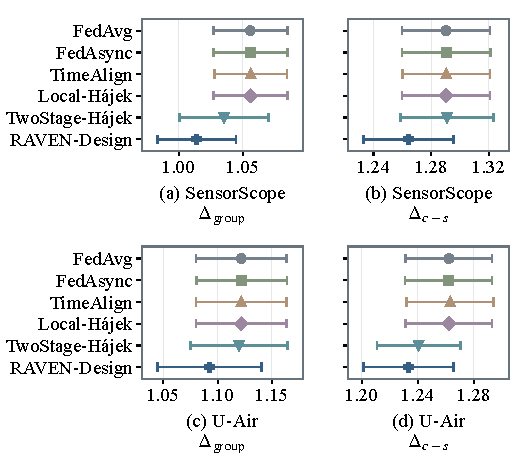
\includegraphics[width=\columnwidth]{fig3_e3_structural_mismatch.pdf}
\caption{Structural mismatch under the frozen station protocols.
Mean $\pm$ sample SD over 20 paired seeds; lower is better.
(a)(b)~SensorScope group/client--stratum mismatch; (c)(d)~U-Air counterparts.
RAVEN-Design is on in both datasets; some active sets differ from
Table~\ref{tab:app_e3_uair}, precluding a matched-support comparison.}
\label{fig:e3_structural}
\end{figure}

\begin{figure}[!htbp]
\centering
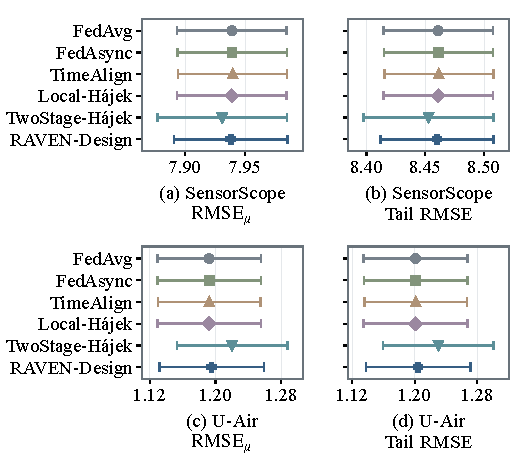
\includegraphics[width=\columnwidth]{fig4_e3_prediction_risk.pdf}
\caption{Prediction error under the frozen station protocols.
Mean $\pm$ sample SD over 20 paired seeds; lower is better.
(a)(b)~SensorScope target/Tail RMSE; (c)(d)~U-Air counterparts.
RAVEN-Design is on; support identities follow Fig.~\ref{fig:e3_structural}.}
\label{fig:e3_prediction}
\end{figure}

\subsection{Four-Block Per-Group RMSE}
\AppNavLabel{app:block_rmse}

Table~\ref{tab:app_block_rmse} reports the four UTC-block scores whose
maximum is $\mathrm{WorstGroupRMSE}$ in
Table~\ref{tab:main_effectiveness}.  The blocks are the public
deployment groups $00$--$06$, $06$--$12$, $12$--$18$, and $18$--$24$~UTC.
The table decomposes the existing prediction endpoint by group.  On both datasets the
worst block is $g=2$ ($12$--$18$~UTC).  The pre-registered under-served
block $g^{\star}$ coincides with that worst block on SensorScope and
does not on U-Air.

\begin{table*}[t]
\centering
\caption{Per-group RMSE across four UTC blocks.
Mean $\pm$ SD over 20 paired seeds; lower is better.
WG denotes $\max_g\mathrm{RMSE}_g$. Both fixed Design settings are shown.}
\label{tab:app_block_rmse}
\footnotesize
\setlength{\tabcolsep}{4pt}
\begin{tabular*}{\textwidth}{@{\extracolsep{\fill}}llccccc}
\toprule
Dataset & Method & $g{=}0$ & $g{=}1$ & $g{=}2$ & $g{=}3$ & WG\\
\midrule
\multirow{6}{*}{SS}
& FedAvg-Window & $7.4912{\pm}0.0464$ & $7.5873{\pm}0.0444$ & $8.6716{\pm}0.0471$ & $8.2084{\pm}0.0460$ & $8.6716{\pm}0.0471$\\
& TwoStage-H\'ajek & $7.4831{\pm}0.0549$ & $7.5795{\pm}0.0523$ & $8.6633{\pm}0.0556$ & $8.2004{\pm}0.0549$ & $8.6633{\pm}0.0556$\\
& FedAU-Window & $7.4887{\pm}0.0512$ & $7.5848{\pm}0.0491$ & $8.6691{\pm}0.0522$ & $8.2059{\pm}0.0510$ & $8.6691{\pm}0.0522$\\
& ObsUse-Window & $7.4815{\pm}0.0517$ & $7.5780{\pm}0.0496$ & $8.6618{\pm}0.0528$ & $8.1988{\pm}0.0516$ & $8.6618{\pm}0.0528$\\
& RAVEN-Design & $7.4903{\pm}0.0479$ & $7.5864{\pm}0.0457$ & $8.6707{\pm}0.0486$ & $8.2075{\pm}0.0476$ & $8.6707{\pm}0.0486$\\
& RAVEN-NoDesign & $7.4907{\pm}0.0474$ & $7.5868{\pm}0.0452$ & $8.6711{\pm}0.0481$ & $8.2079{\pm}0.0470$ & $8.6711{\pm}0.0481$\\
\midrule
\multirow{6}{*}{UA}
& FedAvg-Window & $1.1015{\pm}0.0546$ & $1.1144{\pm}0.0578$ & $1.1690{\pm}0.0692$ & $1.0721{\pm}0.0601$ & $1.1690{\pm}0.0692$\\
& TwoStage-H\'ajek & $1.2009{\pm}0.0623$ & $1.2194{\pm}0.0649$ & $1.2907{\pm}0.0753$ & $1.1800{\pm}0.0670$ & $1.2907{\pm}0.0753$\\
& FedAU-Window & $1.1023{\pm}0.0545$ & $1.1153{\pm}0.0576$ & $1.1701{\pm}0.0689$ & $1.0729{\pm}0.0598$ & $1.1701{\pm}0.0689$\\
& ObsUse-Window & $1.1016{\pm}0.0544$ & $1.1145{\pm}0.0576$ & $1.1692{\pm}0.0689$ & $1.0721{\pm}0.0598$ & $1.1692{\pm}0.0689$\\
& RAVEN-Design & $1.1779{\pm}0.0583$ & $1.1953{\pm}0.0611$ & $1.2630{\pm}0.0716$ & $1.1552{\pm}0.0633$ & $1.2630{\pm}0.0716$\\
& RAVEN-NoDesign & $1.1025{\pm}0.0578$ & $1.1155{\pm}0.0611$ & $1.1703{\pm}0.0734$ & $1.0732{\pm}0.0636$ & $1.1703{\pm}0.0734$\\
\bottomrule
\end{tabular*}
\end{table*}

\subsection{NSW-Traffic Four-Region Protocol Ranking}
\AppNavLabel{app:traffic_four_region}

Table~\ref{tab:traffic_four_region} ranks the same windowed family on
NSW-Traffic under a new public target map: four pre-specified coordinate
regions, not the UTC H1--H4 groups of Table~\ref{tab:main_effectiveness}.
Design is configured on for this block.
$R$, $O$, and $U$ remain Complete-aligned protocol layers.
This block evaluates a distinct public target map on the NSW-Traffic station
traces under the specified selection protocol.
$\mathrm{WorstGroupRMSE}$ is the maximum error over the four regions.
RAVEN-Design versus FedAU-Window and ObsUse-Window stays within
the descriptive $+0.5\%$ worst-group mean-relative point-estimate
tolerance (paired relative $-0.57\%$ and $-0.54\%$).
TwoStage-H\'ajek leads both prediction endpoints and client--stratum alignment;
FedAU-Window leads group alignment.
The block applies the named heuristic to a local map; it does not transfer
the SensorScope/U-Air support statistic.

\begin{table}[!htbp]
\centering
\caption{NSW-Traffic comparison under a four-region target.
Mean $\pm$ SD over ten seeds; 100 windows; lower is better.
Bold marks endpoint minima.}
\label{tab:traffic_four_region}
\footnotesize
\setlength{\tabcolsep}{2.5pt}
\begin{tabular}{@{}lcccc@{}}
\toprule
Method & $\mathrm{RMSE}_{\mu}$ & \shortstack{WorstGroup\\RMSE} &
$\Delta_{\mathrm{group}}$ & $\Delta_{c\text{-}s}$\\
\midrule
FedAvg-Window & \shortstack{$1.0180$\\$\pm0.0089$} & \shortstack{$1.4245$\\$\pm0.0172$} & \shortstack{$0.1877$\\$\pm0.0263$} & \shortstack{$0.9597$\\$\pm0.0290$}\\
TwoStage-H\'ajek & \shortstack{$\mathbf{1.0095}$\\$\pm0.0052$} & \shortstack{$\mathbf{1.4025}$\\$\pm0.0128$} & \shortstack{$0.1908$\\$\pm0.0233$} & \shortstack{$\mathbf{0.8362}$\\$\pm0.0335$}\\
FedAU-Window & \shortstack{$1.0131$\\$\pm0.0078$} & \shortstack{$1.4110$\\$\pm0.0185$} & \shortstack{$\mathbf{0.0606}$\\$\pm0.0192$} & \shortstack{$0.9612$\\$\pm0.0333$}\\
ObsUse-Window & \shortstack{$1.0130$\\$\pm0.0078$} & \shortstack{$1.4106$\\$\pm0.0187$} & \shortstack{$0.0607$\\$\pm0.0192$} & \shortstack{$0.9602$\\$\pm0.0342$}\\
RAVEN-Design & \shortstack{$1.0099$\\$\pm0.0061$} & \shortstack{$1.4029$\\$\pm0.0156$} & \shortstack{$0.1048$\\$\pm0.0242$} & \shortstack{$0.8414$\\$\pm0.0304$}\\
\bottomrule
\end{tabular}

\begin{minipage}{\columnwidth}
\raggedright\footnotesize
$R$, $O$, and $U$ are Complete-aligned protocol layers.
WorstGroupRMSE is the maximum over four coordinate regions, not UTC
H1--H4.  RAVEN-Design is used (Design on).
This comparison uses the four-region target and station-based selection
protocol.  The RMSE superiority contrasts have Holm-adjusted $p>0.05$.
\end{minipage}
\end{table}

\subsection{Balanced No-Harm Control}
\AppNavLabel{app:e1_balanced}

Table~\ref{tab:app_e1_balanced} reports all five paired methods under the balanced
control.  The selected TimeAlign reference has mean
$\mathrm{RMSE}_\mu=7.7108$, while RAVEN-MCS obtains $7.7154$.  RAVEN's
pre-specified mean relative degradation is $0.0599\%$; the one-sided 95\%
upper bound is $0.134\%$, below the pre-specified $3\%$ no-harm margin.
The balanced experiment evaluates this criterion under aligned selection.

\begin{table}[!htbp]
\centering
\caption{Balanced control over the five pre-specified paired seeds.}
\label{tab:app_e1_balanced}
\footnotesize
\setlength{\tabcolsep}{5pt}
\begin{tabular*}{\columnwidth}{@{\extracolsep{\fill}}lcc}
\toprule
Method & $\mathrm{RMSE}_\mu$ & Seeds\\
\midrule
FedAvg-Window & $7.7220\pm0.0289$ & 5 \\
FedAsync-Window & $7.7222\pm0.0287$ & 5 \\
TimeAlign-Agg & $7.7108\pm0.0272$ & 5 \\
TwoStage-H\'ajek & $7.7262\pm0.0291$ & 5 \\
RAVEN-MCS & $7.7154\pm0.0337$ & 5 \\
\bottomrule
\end{tabular*}
\end{table}

\subsection{Complete Risk Non-Interchangeability Statistics}
\AppNavLabel{app:e2_full_stats}

Table~\ref{tab:app_e2_daligned} gives the complete method-level risk-interchangeability summary for
the pre-specified difference-of-differences
$D_{\mathrm{aligned}}=\Delta\mathrm{RMSE}_{\mu}
-\Delta\mathrm{RMSE}_{\rho}$.  The negative mean is stable across all five
methods, and 17--18 of 20 paired seeds are negative.  This supports the
risk-semantic premise that arrival-weighted and deployment-target-weighted
views react differently to the same structured selection shift.

\begin{table}[!htbp]
\centering
\caption{Complete-aligned risk non-interchangeability statistics.
CI denotes the 95\% interval; $p$ is the paired Wilcoxon test of
$D_{\mathrm{aligned}}$ against zero.}
\label{tab:app_e2_daligned}
\footnotesize
\setlength{\tabcolsep}{1pt}
\begin{tabular*}{\columnwidth}{@{\extracolsep{\fill}}lcccc}
\toprule
Method & $D_{\mathrm{aligned}}$ & 95\% CI & \shortstack{Neg.\\seeds} & $p$\\
\midrule
FedAsync-Window & $-0.02115$ & $[-0.03158,-0.01073]$ & 18/20 & $4.83e-04$ \\
FedAvg-Window & $-0.02115$ & $[-0.03158,-0.01071]$ & 18/20 & $4.83e-04$ \\
TimeAlign-Agg & $-0.02137$ & $[-0.03185,-0.01090]$ & 17/20 & $4.83e-04$ \\
RAVEN-MCS & $-0.02088$ & $[-0.03132,-0.01043]$ & 17/20 & $5.86e-04$ \\
TwoStage-H\'ajek & $-0.02120$ & $[-0.03169,-0.01072]$ & 17/20 & $5.86e-04$ \\
\bottomrule
\end{tabular*}
\end{table}


\subsection{Response to Each Selection Layer}
\AppNavLabel{app:e2_layer_matrix}

The six scenarios use five methods and 20 paired seeds each (600 existing
runs).  Table~\ref{tab:e2_layer_matrix} summarizes the final numerical-tie-aware
analysis.  Each range spans the five method-specific mean changes from balanced;
the significant counts retain the existing within-method, within-metric Holm
families over the five non-balanced scenarios.  Signed arrival--target gaps distinguish risk direction from absolute mismatch.

\begin{table*}[t]
\centering
\caption{Risk responses to controlled selection layers on NSW-Traffic.
Changes use the original standardized RMSE units; $\times10^{-3}$ applies to
both range columns. Counts are Holm-significant methods out of five.}
\label{tab:e2_layer_matrix}
\footnotesize
\begin{tabular*}{\textwidth}{@{\extracolsep{\fill}}lrrrr}
\toprule
Scenario & Target change range & Arrival change range & Target significant & Arrival significant\\
\midrule
Balanced & 0 & 0 & -- & --\\
Opportunity only & $[0.057,0.114]$ & $[5.699,5.990]$ & 0/5 & 0/5\\
Observation only & $[0.108,0.157]$ & $[11.018,11.145]$ & 0/5 & 5/5\\
Usable update only & $[0.193,0.245]$ & $[5.472,5.607]$ & 0/5 & 0/5\\
Complete aligned & $[0.757,0.820]$ & $[21.660,22.130]$ & 2/5 & 5/5\\
Complete counteracting & $[0.030,0.059]$ & $[12.447,12.639]$ & 0/5 & 0/5\\
\bottomrule
\end{tabular*}
\end{table*}

\begin{table*}[t]
\centering
\caption{Station-protocol comparison under intermittent opportunities.
Mean $\pm$ SD over 20 paired seeds; lower is better.
RAVEN's fixed Design settings are listed per row.}
\label{tab:int_r_e3}
\footnotesize
\setlength{\tabcolsep}{1pt}
\begin{tabular*}{\textwidth}{@{\extracolsep{\fill}}llcccc}
\toprule
Dataset & Method & $\mathrm{RMSE}_{\mu}$ & \shortstack{WorstGroup\\RMSE} &
$\Delta_{\mathrm{group}}$ & $\Delta_{c\text{-}s}$\\
\midrule
\multirow{5}{*}{SensorScope}
& FedAvg-Window     & \shortstack{$7.9373$\\$\pm0.0960$} & \shortstack{$8.6716$\\$\pm0.0976$} & \shortstack{$1.3411$\\$\pm0.0580$} & \shortstack{$1.5866$\\$\pm0.0445$}\\
& TwoStage-H\'ajek    & \shortstack{$7.9362$\\$\pm0.0956$} & \shortstack{$8.6696$\\$\pm0.0957$} & \shortstack{$1.3558$\\$\pm0.0545$} & \shortstack{$1.5941$\\$\pm0.0415$}\\
& FedAU-Window      & \shortstack{$7.9335$\\$\pm0.1036$} & \shortstack{$8.6678$\\$\pm0.1044$} & \shortstack{$1.3540$\\$\pm0.0541$} & \shortstack{$1.5978$\\$\pm0.0425$}\\
& ObsUse-Window     & \shortstack{$7.9305$\\$\pm0.1047$} & \shortstack{$8.6647$\\$\pm0.1054$} & \shortstack{$1.3560$\\$\pm0.0534$} & \shortstack{$1.5983$\\$\pm0.0421$}\\
& RAVEN-Design & \shortstack{$7.9407$\\$\pm0.0957$} & \shortstack{$8.6746$\\$\pm0.0972$} & \shortstack{$\mathbf{1.3272}$\\$\pm0.0607$} & \shortstack{$1.5859$\\$\pm0.0443$}\\
\midrule
\multirow{6}{*}{U-Air}
& FedAvg-Window     & \shortstack{$1.1121$\\$\pm0.0873$} & \shortstack{$1.1682$\\$\pm0.1022$} & \shortstack{$1.3141$\\$\pm0.0679$} & \shortstack{$1.5786$\\$\pm0.0602$}\\
& TwoStage-H\'ajek    & \shortstack{$1.1555$\\$\pm0.1027$} & \shortstack{$1.2179$\\$\pm0.1079$} & \shortstack{$1.4393$\\$\pm0.0613$} & \shortstack{$1.5694$\\$\pm0.0631$}\\
& FedAU-Window      & \shortstack{$1.1126$\\$\pm0.0845$} & \shortstack{$1.1689$\\$\pm0.0985$} & \shortstack{$1.3319$\\$\pm0.0690$} & \shortstack{$1.5951$\\$\pm0.0597$}\\
& ObsUse-Window     & \shortstack{$1.1126$\\$\pm0.0853$} & \shortstack{$1.1689$\\$\pm0.0995$} & \shortstack{$1.3304$\\$\pm0.0693$} & \shortstack{$1.5947$\\$\pm0.0604$}\\
& RAVEN-Design & \shortstack{$1.1528$\\$\pm0.1005$} & \shortstack{$1.2148$\\$\pm0.1040$} & \shortstack{$1.4134$\\$\pm0.0725$} & \shortstack{$\mathbf{1.5632}$\\$\pm0.0663$}\\
& RAVEN-NoDesign & \shortstack{$1.1120$\\$\pm0.0880$} & \shortstack{$1.1680$\\$\pm0.1031$} & \shortstack{$\mathbf{1.2959}$\\$\pm0.0746$} & \shortstack{$1.5672$\\$\pm0.0638$}\\
\bottomrule
\end{tabular*}
\end{table*}

\subsection{Under-Served-Block Validation}
\AppNavLabel{app:underserved_block}
On validation only, aggregate target and opportunity mass to four UTC blocks
and freeze $g^\star=\arg\max_b(\mu_b^{\mathrm{blk}}-
\pi_b^{\mathrm{opp},4})$: block 2 on SensorScope and 3 on U-Air, with gaps
$.114/.172$.  The required improvement against both FedAU and ObsUse is
$-.5\%$.  Observed $+.05\%/+.15\%$ and $-.44\%/-.27\%$ miss that criterion
while meeting no-harm (Supplementary Table~\ref{tab:underserved_block}).  

\begin{table}[!htbp]
\centering
\caption{Validation RMSE in under-served UTC blocks.
Relative changes (\%) over ten paired validation seeds versus
FedAU-Window/ObsUse-Window; negative favors RAVEN.
Design is on for SensorScope and off for U-Air.
Improvement/no-harm thresholds are $\le-0.5\%$/$\le+0.5\%$.}
\label{tab:underserved_block}
\setlength{\tabcolsep}{3.5pt}
\begin{tabular}{lcccc}
\toprule
Dataset & $g^{\star}$ (UTC) & vs FedAU & vs ObsUse & Win / no-harm\\
\midrule
SensorScope & 2 (12--18) & $+0.05\%$ & $+0.15\%$ & No / Yes\\
U-Air & 3 (18--24) & $-0.44\%$ & $-0.27\%$ & No / Yes\\
\bottomrule
\end{tabular}
\end{table}











\subsection{Intermittent Opportunity Protocol}
\AppNavLabel{app:int_r}




Table~\ref{tab:main_effectiveness} uses always-on Complete-aligned opportunity.
This ranking keeps the SensorScope and U-Air station arrays, the public
four-block $\boldsymbol\mu$, and the Complete-aligned $O$/$U$ layers, and
replaces protocol $R$ by a client-window bit $A_{k,t}$. $A_{k,t}=0$ writes
no opportunity event; $A_{k,t}=1$ leaves the existing $O$/$U$ path unchanged.
Occupancy is a two-state Markov chain, independent across $K=8$ clients, with
mean active fraction $0.425$ from the published T-Drive scalar in
Section~\ref{subsec:eval_rq1}. The same $(\alpha,\beta)$ is used on both
datasets. T-Drive GPS is not overlaid. Design is not retuned on these RMSE
values; both settings in Table~\ref{tab:main_effectiveness} are reported. The
coverage Gate in Section~\ref{subsec:limitations} is not used.

A declared Goh--Barab\'asi burstiness of $+0.38$ was screened to keep
single-seed active fractions in $[0.35,0.50]$. The selected chain
($\alpha\approx0.775$, $\beta\approx0.837$) has pooled burstiness about
$0.20$, so the block matches the published T-Drive active fraction, not
T-Drive burstiness, and it is not a taxi process.

Table~\ref{tab:int_r_occ} covers seeds $30001$, $30010$, and $30020$. Seed
$30001$ has mean active fraction in $[0.35,0.50]$ on both datasets.
Four-block $\mathrm{TV}(\pi^{\mathrm{opp}},\boldsymbol\mu)$ stays above the
pre-registered $0.05$ threshold ($0.309$ SensorScope, $0.225$ U-Air), so
intermittent occupancy does not remove the mismatch in
Table~\ref{tab:main_effectiveness}.

\begin{table}[!htbp]
\centering
\caption{INT-R occupancy on shared event traces.
Eight logical clients; burstiness is Goh--Barab\'asi on pooled inter-active
gaps. $\mathrm{TV}$ uses $A=1$ risk sets and training units only.}
\label{tab:int_r_occ}
\footnotesize
\begin{tabular}{lcccc}
\toprule
Dataset & Seed & Active frac. & Burstiness & $\mathrm{TV}(\pi^{\mathrm{opp}},\boldsymbol\mu)$\\
\midrule
SensorScope & 30001 & $0.453$ & $0.198$ & $0.309$\\
SensorScope & 30010 & $0.433$ & $0.223$ & $0.300$\\
SensorScope & 30020 & $0.394$ & $0.251$ & $0.271$\\
U-Air & 30001 & $0.495$ & $0.263$ & $0.225$\\
U-Air & 30010 & $0.428$ & $0.190$ & $0.275$\\
U-Air & 30020 & $0.403$ & $0.201$ & $0.205$\\
\bottomrule
\end{tabular}
\end{table}

Table~\ref{tab:int_r_e3} ranks the same methods as
Table~\ref{tab:main_effectiveness} on those traces ($20$ paired seeds).
Three always-on conclusions survive.  (i)~Four-block
$\mathrm{WorstGroupRMSE}$ remains within the descriptive $+0.5\%$
tolerance versus FedAU-Window
and ObsUse-Window: SensorScope paired relative
change $+0.08\%$ and $+0.12\%$; U-Air $-0.10\%$ and $-0.10\%$.  Holm tests
against those two have adjusted $p>0.05$.  (ii)~Design on for U-Air
still worsens the primaries relative to RAVEN-NoDesign
(paired $+3.65\%$ $\mathrm{RMSE}_{\mu}$ and $+4.07\%$
$\mathrm{WorstGroupRMSE}$; $+9.14\%$ $\Delta_{\mathrm{group}}$), while
slightly improving $\Delta_{c\text{-}s}$ ($-0.26\%$).  The always-on
reversal was about $7\%$ on the primaries; the sign is unchanged.
(iii)~SensorScope $\Delta_{\mathrm{group}}$ remains lower for
RAVEN-Design than for FedAvg (paired $-1.04\%$).

The thinner opportunity process changes the structural effects.  On
SensorScope, the $\Delta_{c\text{-}s}$ contrast with FedAvg shrinks to
$-0.05\%$, and removing Design changes $\Delta_{\mathrm{group}}$ by
$+0.05\%$; neither contrast is significant ($p>0.05$).
Every method also has higher absolute $\Delta_{\mathrm{group}}$ than in
Table~\ref{tab:main_effectiveness}, about $1.33$ versus $1.01$ on SensorScope.



\section{Mechanism Analysis and Numerical Calibration Details}
\AppNavLabel{app:rq2_details}
Mechanism conditions and numerical calibration details support RQ2.

\subsection{Local-H\'ajek Weight Cancellation}
\AppNavLabel{app:local_hajek}

\begin{table}[!htbp]
\centering
\caption{Within-client weight constancy.}
\label{tab:app_local_hajek}
\footnotesize
\setlength{\tabcolsep}{5pt}
\begin{tabular*}{\columnwidth}{@{\extracolsep{\fill}}lcc}
\toprule
Dataset & Effective client-windows & Weight range\\
\midrule
SensorScope & 6070 & $0$\\
U-Air & 3596 & $0$\\
\midrule
Total & 9666 & $0$\\
\bottomrule
\end{tabular*}
\end{table}


The equality between Local-Hajek and FedAvg in the formal SensorScope/U-Air
blocks is protocol-specific and does not imply general
equivalence. Table~\ref{tab:app_local_hajek} covers
9666 effective client-windows: 6070 on SensorScope and
3596 on U-Air. In every effective client-window, the realized
within-client correction-weight range is 0.



The collapse follows directly from the normalized local objective.  Let
$\mathcal I_{k,r}^{+}$ be the records retained by an effective client-window
and let $N_{k,r}^{+}=|\mathcal I_{k,r}^{+}|$.  If the realized first-stage
weight is constant over that set, i.e.,
$a_{k,r,i}=a_{k,r}>0$ for all $i\in\mathcal I_{k,r}^{+}$, then
\begin{equation}
 \overline a_{k,r,i}
 =
 \frac{a_{k,r}}
 {N_{k,r}^{+}a_{k,r}}
 =
 \frac{1}{N_{k,r}^{+}}.
 \label{eq:app_local_hajek_uniform}
\end{equation}
Consequently,
\begin{equation}
 \widehat F^H_{k,r}(\theta)
 =
 \frac{1}{N_{k,r}^{+}}
 \sum_{i\in\mathcal I_{k,r}^{+}}
 \frac{1}{2}
 \left(
 f_\theta(i;C_i^{\mathrm{dep}})-Z_{k,r,i}
 \right)^2,
 \label{eq:app_local_hajek_collapse}
\end{equation}
which is exactly the uniform local objective used by the matched FedAvg
backbone in these realized windows.
\qed

The derivation accounts for the observed numerical equality when within-window
correction weights are constant. Heterogeneous weights are a different case.


\subsection{Within-Stratum Observation Heterogeneity}
\AppNavLabel{app:f1_mechanism}

The within-stratum heterogeneity construction changes the observation probability to
$p_i=\operatorname{clip}(\operatorname{sigmoid}(b_{0,b}+\theta_O z_i),.05,.95)$,
where $z_i\in\{-1,0,1\}$ is the time-index tercile of a training unit within
its opportunity stratum.  The block intercept $b_{0,b}$ preserves the original
block mean, .35 or .1925.  It uses no current response value.  Thus the
intervention introduces within-stratum covariate dependence, not general MNAR
selection.  At $\theta_O=0$ the copied selection traces coincide with the
original construction; at $\theta_O=1$ they are regenerated with the same
opportunity, delivery process, seeds, splits, and target maps.

\begin{table}[!htbp]
\centering
\caption{Within-stratum observation-probability diversity. Distinct probabilities are
counted per opportunity stratum; entries are stratum means. The block marginal
is preserved by construction.}
\label{tab:f1_mechanism}
\footnotesize
\begin{tabular*}{\columnwidth}{@{\extracolsep{\fill}}lrr}
\toprule
Dataset & $\theta_O=0$ & $\theta_O=1$\\
\midrule
SensorScope & 1.00 & 2.76\\
U-Air & 1.00 & 2.83\\
\bottomrule
\end{tabular*}
\end{table}

The estimated-propensity arm keeps the original covariates. The true-$p$ arm
replaces only the atomic observation propensity, retaining estimated $q$ and
Design on. Its local inverse weights can vary across time terciles, while a
stratum-constant factor cancels under local H\'ajek normalization. Block
observation means stay at .35 or .1925.

\subsection{Design-Induced Support Changes}
\AppNavLabel{app:design_provenance}

The end-to-end Design comparison in Section~\ref{subsec:rq1_alignment} exhibits an endpoint
trade-off on U-Air. Across 774 paired windows, full RAVEN and w/o-Design share
opportunity, observation, usable-update, and registration events. Removing the
Design ratio changes positive-mass calibration support, so the end-to-end contrast
includes support changes as well as weight changes.


\FloatBarrier
\subsection{Numerical Feasibility of Calibration}
\AppNavLabel{app:p2_diagnostics}

Theorem~1 concerns the mathematical program. Numerical checks test stored
allocations against calibration constraints where the required state is logged.
Table~\ref{tab:app_p2_coverage}
summarizes the dataset-level certificate coverage.

\begin{table}[!t]
\centering
\caption{Calibration feasibility-certificate coverage in the formal protocol blocks.}
\label{tab:app_p2_coverage}
\footnotesize
\setlength{\tabcolsep}{4pt}
\begin{tabular*}{\columnwidth}{@{\extracolsep{\fill}}lcccc}
\toprule
Dataset & Runs & Mean windows & Range & Status\\
\midrule
SensorScope & 180 & 93.85 & 88--98 & Certified \\
U-Air & 180 & 72.61 & 63--79 & Certified \\
\bottomrule
\end{tabular*}
\end{table}

The solver log contains 778 numerical-inaccuracy warnings on 85 formal runs.
Table~\ref{tab:app_p2_warning_audit} covers 6438 active calibration windows; the maximum constraint
residual is $2.686\times10^{-8}<10^{-7}$, which certifies feasibility.
Where the invocation state is reconstructable, CLARABEL and SCS typically
match to $10^{-8}$ in $\ell_1$; the worst window differs by $0.0056$ in
allocation.
The pre-specified solver-discrepancy rule uses $10^{-4}/10^{-3}$ thresholds.
Stored calibration outputs were not re-solved.

\begin{table}[!t]
\centering
\caption{Numerical feasibility of warning-affected calibration allocations.}
\label{tab:app_p2_warning_audit}
\footnotesize
\setlength{\tabcolsep}{5pt}
\begin{tabular*}{\columnwidth}{@{\extracolsep{\fill}}lc}
\toprule
Quantity & Result\\
\midrule
Numerical-inaccuracy warnings & 778\\
Affected formal runs & 85\\
Evaluated active windows & 6438\\
Maximum constraint residual & $2.686\times10^{-8}$\\
Feasibility & Certified\\
Optimality certificate in stored logs & Unavailable\\
\bottomrule
\end{tabular*}
\end{table}


\subsection{Calibration Contrasts and Debt Sensitivity}
\AppNavLabel{app:trained_rule_probe}
\AppNavLabel{app:kappa_probe}

\AppNavLabel{app:matched_support_contrasts}

The following group-TV changes use percentage points (pp); intervals are
95\% seed-paired bootstrap confidence intervals. Projection versus the direct
corrected reference gives 1.188 pp [0.956, 1.409] on SensorScope and
1.399 pp [1.019, 1.782] on U-Air. Projection versus Uniform gives
0.768 pp [0.563, 0.970] and 0.286 pp [0.098, 0.471], respectively.
U-Air's latter effect is 0.170 pp on tuning seeds and 0.402 pp on report seeds.
SensorScope's independent same-support projected Design-on/off contrast is
0.922 pp [0.721, 1.141], not additive with projection versus Uniform.
The direct-reference group mismatches are 1.03533 and 1.11961, respectively.
For full calibration versus projection, the prediction tests give
$p_{\mathrm{Holm}}=1$ on SensorScope and a minimum of 0.120 on U-Air,
using the common saved-parameter scoring rule.


At tuned $\kappa=1000$, projection-with-debt reduces group-TV versus projection
by $1.347$ pp on SensorScope and $.580$ pp on U-Air (Holm $\approx10^{-5}$).
SensorScope's gain at the pre-specified debt coefficient is $.0073$ pp,
within the practical band.
Projection's maximum endpoint discrepancy across 240 runs is
$\varepsilon_{\mathrm{impl}}=2.42\times10^{-5}$ in $\Delta$ units ($.00121$ pp):
17\% of the debt effect at the pre-specified coefficient, $.13\%$ of the
Design contrast, and $.16\%$ of the projection contrast. Primal residuals reach $6.66\times10^{-16}$ against tolerance
$10^{-13}$, while stationarity residuals reach $.667$ against $10^{-12}$.
Comparator objective gaps exceed $10^{-12}$ in 7 of 200 sampled windows,
with maximum $9.64\times10^{-12}$. These diagnostics separate numerical
feasibility and endpoint agreement from exact optimality.



\subsection{Runtime under Risk-Semantic Workloads}
\AppNavLabel{app:runtime}

In Table~\ref{tab:app_runtime}, the ``all scenarios'' column aggregates six
risk-semantic scenarios and 20 seeds (120 runs per method); the Complete-aligned column
contains 20 runs per method.

\begin{table}[!t]
\centering
\caption{Runtime on the risk-semantic workloads.
Wall-clock seconds per run, mean $\pm$ SD.}
\label{tab:app_runtime}
\footnotesize
\setlength{\tabcolsep}{3.5pt}
\begin{tabular*}{\columnwidth}{@{\extracolsep{\fill}}lcc}
\toprule
Method & All scenarios & Complete-aligned\\
\midrule
FedAvg-Window & $71.426\pm5.105$ & $69.278\pm2.287$ \\
FedAsync-Window & $71.418\pm4.863$ & $70.186\pm3.531$ \\
TimeAlign-Agg & $71.244\pm5.225$ & $69.217\pm2.554$ \\
TwoStage-H\'ajek & $71.781\pm8.017$ & $69.829\pm3.670$ \\
RAVEN-MCS & $72.669\pm4.243$ & $71.070\pm1.292$ \\
\bottomrule
\end{tabular*}
\end{table}

The runtime rows in Table~\ref{tab:app_runtime} summarize completed runs on the
specified workload sizes and selection scenarios.

\section{Target Support, Target Maps, and Reference Sensitivity}
\AppNavLabel{app:rq3_details}
Support geometry, target maps, and reference sensitivity address RQ3.

\subsection{Instantaneous Arrival-Support Geometry}
\AppNavLabel{app:arrival_support}

The rows use the formal complete-aligned logs for NSW-Traffic, SensorScope,
and U-Air, seeds $30001$--$30020$. A nonempty close keeps $U=1$ attempts;
one client keeps the largest downloaded version. That attempt is one column
of $M^{\mathrm{arr}}$: the frozen UTC block of its observed units on Traffic,
and the spatial-and-block group named by its opportunity stratum on
SensorScope and U-Air. Empty closes are dropped ($5382$ remain). U-Air
contributes $1515$ closes; the $1402$ Design-on active windows in the main
text are a different set.

Positive target mass splits into missing mass ($n_g=0$), narrow-range mass
($n_g>0$, $W_g<.01$), and adjustable mass ($W_g\ge.01$), with
$\overline\alpha=\min\{1,\max\{.5,1/K\}\}$ and $\overline E=\min\{3,K\}$.
For $K\le 3$ the feasible set is uniform, so adjustable mass is $0$.
$d_{\mathrm{simplex}}$, $d_{\mathrm{cap}}$, $d_{\mathrm{ESS}}$, and
$d_{\mathcal C}$ minimize $\|M^{\mathrm{arr}}\alpha-\mu\|_1$ on the simplex,
under the cap, under $\sum_k\alpha_k^2\le 1/\overline E$, and under both.
These are $\ell_1$ distances, separate from the squared $\ell_2$ gap
$d_r^{\mathrm{feas}}$ in Appendix~\ref{app:supp_calibration_geometry}.

\begin{proposition}[Arrival-support simplex distance]
\label{prop:arrival_simplex}
If every column of $M$ is a basis vector, $\mu_g\ge 0$, and $\sum_g\mu_g=1$,
then on the simplex
$\min_{\alpha}\|M\alpha-\mu\|_1=2\mu_{\mathrm{miss}}$,
where $\mu_{\mathrm{miss}}$ is the target mass on groups with no column.
\end{proposition}

\begin{proof}
Absent groups contribute $\mu_{\mathrm{miss}}$, and present groups must carry
total mass $1$, so they sit at least $\mu_{\mathrm{miss}}$ above their combined
target. Matching each present target and placing the residual on one present
client attains the bound. The same value under the cap and the ESS bound is
measured in Table~\ref{tab:arrival_support}; it is not claimed for arbitrary caps.
\end{proof}

The four minima agree through $10^{-11}$, and all $2966$ closes with
$K\le 3$ have adjustable mass $0$. Table~\ref{tab:arrival_support} gives the
common distance. Seeds are averaged inside a stratum, then averaged with
equal weight. For $K>3$, adjustable mass has descriptive interval
$[2.220\%,2.283\%]$ on SensorScope and $[2.938\%,3.020\%]$ on U-Air
($10{,}000$ resamples, seed $20261019$).

\begin{table}[!htbp]
\centering
\caption{Arrival-log geometry. Masses are percentages of positive target
mass. L1 is the shared minimum $\ell_1$ distance on $M^{\mathrm{arr}}$.}
\label{tab:arrival_support}
\footnotesize
\setlength{\tabcolsep}{2.5pt}
\begin{tabular}{llrrrrr}
\toprule
Dataset & $K$ & Windows & Miss. & Narrow & Adj. & L1\\
\midrule
Traffic & $\le 3$ & 294 & 75.000 & 25.000 & 0 & 1.5000\\
Traffic & $>3$ & 1696 & 75.000 & 25.000 & 0 & 1.5000\\
SensorScope & $\le 3$ & 1475 & 98.916 & 1.084 & 0 & 1.9783\\
SensorScope & $>3$ & 402 & 97.748 & 0 & 2.252 & 1.9550\\
U-Air & $\le 3$ & 1197 & 98.551 & 1.449 & 0 & 1.9710\\
U-Air & $>3$ & 318 & 97.024 & 0 & 2.976 & 1.9405\\
\bottomrule
\end{tabular}
\end{table}

Every Traffic close covers one UTC block, so $75\%$ of the target is absent,
the present block has range zero, and the minimum distance is $1.5$. For
$K>3$, SensorScope and U-Air leave $2.252\%$ and $2.976\%$ adjustable. The cap
and ESS bound do not raise that one-close minimum. Cross-window mismatch and
RMSE are separate questions.

Under arrival-time consumption, an attempt still inside the staleness bound
at its arrival close is consumed there. On these three traces the hold set
matches the arrival set in every nonempty window, so the adjustable-mass
difference is zero. Retaining an update past that close is a different rule,
and this comparison did not train it.

\subsection{City Scanner Target Maps and Zero-Mass Handling}
\AppNavLabel{app:cityscanner_sixarm}

The six-arm visit-occupancy comparison uses controlled $O/U$ and ten traces
with model seeds $s,s+100000,s+200000$: 150 newly trained and 30 reused runs.
Maps use public locations, calendar strata and test-region shares before
training, without responses/errors. Table~\ref{tab:cityscanner_sixarm}
summarizes ten within-trace model-seed means.

\begin{table}[!htbp]
\centering
\caption{Client--stratum gaps across City Scanner target maps.
Mean $\pm$ SD over ten trace means, each using three model seeds.
Targets are arm-specific, so gaps do not rank common-target alignment.}
\label{tab:cityscanner_sixarm_cs}
\footnotesize
\begin{tabular}{lr}
\toprule
Method / target map & $\Delta_{c\text{-}s}$\\
\midrule
FedAvg / count & $0.8123{\pm}0.0191$\\
RAVEN-NoDesign & $0.7880{\pm}0.0254$\\
RAVEN-control & $0.5676{\pm}0.0311$\\
RAVEN-floor & $0.7892{\pm}0.0235$\\
RAVEN-M1$\mu$ & $1.4060{\pm}0.0168$\\
RAVEN-M2$\mu$ & $1.4348{\pm}0.0147$\\
\bottomrule
\end{tabular}
\end{table}

Count-weighted FedAvg and RAVEN-NoDesign omit the target ratio.
RAVEN-control has 1164 keys, 812 zero; RAVEN-floor replaces zeros with
$4.78469\times10^{-4}$, the smallest positive mass, and renormalizes,
changing group marginals. RAVEN-M1$\mu$/RAVEN-M2$\mu$ use ACS population/NYC~311
shapes on these keys, rescaled within region to the common target (70/33 zeros).
All maps cover the 959 risk-set keys.

For $d_t=R_{\mathrm{ctrl},t}/R_{\mathrm{floor},t}-1$ on within-trace mean RMSE,
Hodges--Lehmann gives $-.019\%$ (paired Wilcoxon $p=.922$).
Hierarchical resampling of traces and their model seeds gives the 95\%
percentile interval $[-1.89\%,+12.28\%]$, including zero but extending above
the $2\%$ equivalence band. Group-gain retention is
$(\overline\Delta_{\mathrm{FedAvg}}-\overline\Delta_{\mathrm{floor}})/
(\overline\Delta_{\mathrm{FedAvg}}-\overline\Delta_{\mathrm{ctrl}})=1.0194$.

Registered floor/M1$\mu$/M2$\mu$ versus FedAvg chains use one-sided paired
Wilcoxon tests of within-trace three-seed mean group differences (H1). All
ten traces improve (individual $p=.0009765625$) and reject at family-level
$.05$ (initial weights $1/3$, Holm redistribution $1/2$). Prediction
non-inferiority (H2) needs a Wilcoxon-inverted one-sided upper bound below
$2\%$; the bounds $3.83/4.14/8.15\%$ fail, so superiority (H3) is untested.
The secondary Holm family (M1/control, M2/control, floor/NoDesign, six-arm
dose-response slope) has no significant member. All traces stay in the
primary analysis. Trace 32005's control/NoDesign cost recurs on five model
seeds; dropping it only in a sensitivity pass gives $[-2.32\%,+3.53\%]$,
still inconclusive. All-trace diagnostic power at $2\%$ is $.151$.

\subsection{Offline Configuration and Retrospective Trade-offs}
\AppNavLabel{app:cityscanner_phi}
For block $r$, $n_r$ counts unique training units and $n_r^{\mathrm{zero}}$
those with a zero-target attached client--stratum key. The offline rule is
\begin{equation}
\rho_r=\frac{n^{\mathrm{zero}}_r}{n_r},
\qquad
D_r=\mathrm{on}\iff\rho_r=0 .
\label{eq:design_gate}
\end{equation}
Table~\ref{tab:scd_phi_freeze} distinguishes its lookup objects. A pre-window
configuration requires the catalogue and public lookup to exist then;
current outcomes and the coverage Gate do not select Design. The counts
use no $Y$ or RMSE, establish neither target-positive support nor input
availability timing, and differ from U-Air's $25.5\%$ EventTrace occurrence.
For measured endpoints $M_{e,r}(D)$,
$e\in\{\Delta_{\mathrm{group}},\Delta_{c\text{-}s},\mathrm{RMSE}_{\mu},\mathrm{Tail}\}$,
and nonnegative weights $w_e$, the retrospective chart is
\begin{equation}
\begin{aligned}
\widehat J_r(D)&=\sum_{e\in\mathcal{E}}w_e\,\frac{M_{e,r}(D)}{M_{e,r}(\mathrm{on})},\\
D_r^{\star}&=\arg\min_{D\in\{\mathrm{on},\mathrm{off}\}}\widehat J_r(D),
\end{aligned}
\label{eq:design_switch}
\end{equation}
Using structural terms alone gives U-Air indifference at $w_c/w_g=1.39$.
This chart is not the experiments' online rule. Both fixed Design settings
remain reported where their trade-off matters.

\begin{table}[!htbp]
\centering
\caption{Offline zero-target counts for attached clients.
Frozen $\pi^{\mathrm{tar}}(k(i),s(i))$; missing keys count as zero.
Design uses rule~\eqref{eq:design_gate}.}
\label{tab:scd_phi_freeze}
\footnotesize
\setlength{\tabcolsep}{1pt}
\begin{tabular*}{\columnwidth}{@{\extracolsep{\fill}}lcccc}
\toprule
Block & $n_{\mathrm{train}}$ & $n_{\mathrm{zero}}$ & coverage & Design \eqref{eq:design_gate}\\
\midrule
SensorScope (Table~\ref{tab:main_effectiveness}) & $10285$ & $0$ & $0$ & on\\
U-Air (Table~\ref{tab:main_effectiveness}) & $5688$ & $2016$ & $35.4\%$ & off\\
T-Drive hybrid (Table~\ref{tab:tdrive_hybrid}) & $285659$ & $135268$ & $47.4\%$ & off\\
NSW-Traffic four-region (Table~\ref{tab:traffic_four_region}) & $18576$ & $0$ & $0$ & on\\
City Scanner NYC {PM}$_{2.5}$ (Table~\ref{tab:cityscanner_hybrid}) & $9343$ & $0$ & $0$ & on\\
\shortstack[l]{City Scanner Pilot 2\\measured $O$ (Table~\ref{tab:cityscanner_p2_measured_o})} & $10141$ & $0$ & $0$ & on\\
\bottomrule
\end{tabular*}
\end{table}

Lookup objects differ: test-split client--stratum mass
$\pi^{\mathrm{tar}}_{k,s}$ on SensorScope/U-Air, test-stratum frequency on
T-Drive, and a four-region freeze on NSW-Traffic. City Scanner assigns
positive test-group shares $\mu_{h(i)}$ to training atoms, rather than
checking target-positive pairs; its zero count is not the SensorScope/U-Air
support check.

\subsection{Support and Stabilization Conditions}
\AppNavLabel{app:a5_a6_audit}
Proposition~\ref{prop:practical_plugin} uses A1, A4, A5, A6b and shared-state,
positive-mass conditions; A6a suffices for zero stabilization error but is not required by the bound. Twenty seeds yield 16000/12800 SensorScope/U-Air
client-windows (12346/9760 observed), with
$p_{\min}=q_{\min}=.05$, $\pi_{\min}=10^{-6}$, $a_{\max}=20$, $d_{\max}=10$.
The table uses true rather than unavailable estimated margins. Across 28800
records, observation probabilities are block-constant $.1925/.35$;
usable probability is shared by at most four risk units, without label dependence.

\begin{table}[!htbp]
\centering
\caption{Support and stabilization on station traces.
Floor/ceiling activation percentages use observed client-windows.
The mass minimum omits opportunity correction. Composite ceilings and
$\varepsilon_{\mathrm{stab}}$ use true margins on active support over 20
Design-on runs; the latter reports median/p95/max.}
\label{tab:app_a5_a6_audit}
\footnotesize
\setlength{\tabcolsep}{3pt}
\begin{tabular*}{\columnwidth}{@{\extracolsep{\fill}}llcc}
\toprule
 & Sub-condition & SensorScope & U-Air\\
\midrule
A5 & $\min \pi^{\mathrm{opp}}>0$ & $6.33\times10^{-4}$ & $1.39\times10^{-3}$\\
A5 & $\min p^{\mathrm{obs}}\ge p_{\min}$ & $0.1925$ & $0.1925$\\
A5 & $\min q^{\mathrm{use}}>0$ (observed) & $0.0055$ & $0.0055$\\
A5 & Obs./use mass minimum & $5.521$ & $16.89$\\
\midrule
A6a & $q_{\min}$ floor activation & $5.22\%$ & $5.18\%$\\
A6a & $d_{\max}$ ceiling activation & $24.22\%$ & $23.75\%$\\
A6a & $\max 1/p^{\mathrm{obs}}$, Design off & $5.195$ & $5.195$\\
A6a & $\max \zeta/p^{\mathrm{obs}}$, Design on & $19.26$ & $\mathbf{23.47}$\\
\midrule
A6a & $\varepsilon_{\mathrm{stab}}$ med/p95/max & $0/0.07/0.55$ & $0/0.05/0.68$\\
\bottomrule
\end{tabular*}
\end{table}

\noindent\textbf{Support and mass.}
Minimum observed usable margin is $.0055$. Pre-opportunity mass minima
$5.521/16.89$ differ from full-reference mass. Zero usable margins occur
in $22.84\%/23.75\%$ of all client-windows but none of 12346/9760 observed
records: never-observed/usable cells are outside estimator support.

\noindent\textbf{Stabilization and conditions.}
Including unobserved cells, $q^{\mathrm{use}}<1/d_{\max}$ occurs in
$41.52\%/41.86\%$. Table maxima $19.26/23.47$ exceed ceiling $20$ only for
$2.74\%$ of active U-Air client-windows; ceiling $40$ would contain both.
True-margin stabilization error is positive on $10.7\%/11.1\%$ of active
windows (median $0$, maximum $.553/.680$), mainly from usability with an
additional Design-on opportunity contribution. The worst-case
$L_\pi\le2\times10^{13}$ is loose. Shared $\mathcal A_r,M_r,\mathcal C_r$,
positive reference mass and A6b remain conditions: saved states omit
active-set lists and estimated margins, preventing A6b and plug-in-error checks.

\subsection{Reference and Prediction Sensitivity}
\AppNavLabel{app:reference_sensitivity}
On 20 paired seeds, true observation/usability margins change calibrated
RMSE by $-.008\%$ ($[-.041,+.025]\%$) on SensorScope and $+.040\%$
($[-.090,+.171]\%$) on U-Air. Three U-Air members stay within $.3\%$;
TwoStage-H\'ajek is $2.04\%$ above its oracle counterpart ($[1.33,2.75]\%$).
Reference $\ell_1$ perturbations have median $.077$, maximum $1.15$.
For $H=(\mathrm{RMSE}_{\mu}(\mathrm{FedAvg})-\mathrm{RMSE}_{\mu}(\mathrm{oracle}))/
\mathrm{RMSE}_{\mu}(\mathrm{FedAvg})$, varying opportunity tilt, tail observation,
capacity and target yields SensorScope effects $[-.03\%,+.08\%]$ (detectable
$.17$--$.36$ pp). U-Air's 270 runs/45 traces give $|H|\le.217\%$ with
zero-containing intervals; $.70$--$.80$ pp detection leaves $.5\%$ improvement
unresolved. These are evaluated configurations, not predictive optima.

\subsection{Target-Concentration Sensitivity}
\AppNavLabel{app:target_concentration}



Table~\ref{tab:target_concentration} multiplies region1's prior mass by
$\kappa_{\mathrm{tar}}$ then renormalizes, retaining backbone, two local steps
and server rule. Local-H\'ajek versus full-path RAVEN-SimOracle uses generator
observation and Monte Carlo usability probabilities. Baseline runs are reused;
$5$ uses the four-arm experiment; $10$ and single-region conditions each add
20 paired seeds. This multiplier differs from debt strength $\kappa$.



\begin{table}[!htbp]
\centering
\caption{Target-concentration sensitivity on NSW-Traffic.
$D$ is control minus oracle test RMSE in the original standardized units;
relative gain is $100\overline D/\overline{\mathrm{RMSE}}_{\mathrm{control}}$.
Intervals and MDE use seed-paired analysis.}
\label{tab:target_concentration}
\footnotesize
\setlength{\tabcolsep}{2.2pt}
\begin{tabular}{lrrrr}
\toprule
$\kappa_{\mathrm{tar}}$ & Top region & $\overline D$ [95\% CI] & MDE$_{80}$ & Gain (\%)\\
\midrule
1 & $0.256$ & \shortstack{$0.000013$\\$[-0.000099,0.000148]$} & $0.000197$ & $0.0013$\\
5 & $0.632$ & \shortstack{$0.000228$\\$[0.000055,0.000422]$} & $0.000289$ & $0.0225$\\
10 & $0.775$ & \shortstack{$0.000462$\\$[0.000241,0.000708]$} & $0.000367$ & $0.0454$\\
Single region & $1.000$ & \shortstack{$0.000994$\\$[0.000685,0.001337]$} & $0.000511$ & $0.0970$\\
\bottomrule
\end{tabular}
\end{table}

At $10$ and the single-region limit, intervals exclude zero and means exceed
MDE; at $5$ only intervals exclude zero. All effects remain below the $2\%$
criterion, so target dilution alone does not explain this configuration's small gain.

\section{Coverage-Controlled Variant under Availability Stress}
\AppNavLabel{app:certificate_audit}
Conditional diagnostic proofs are in Appendix~\ref{app:agg_coverage_proofs}.

\label{subsec:limitations}

Table~\ref{tab:certificate_stress} and Fig.~\ref{fig:certificate_audit}
evaluate a coverage-controlled Design variant with
$\mathrm{Design}_t=\mathrm{Gate}_t$, rather than the main method's pre-window
Design configuration and diagnostic-only Gate. Pooled CERTIFIED validity is
$0.959$ with zero false-safe openings. The stable-block guarantee in
Section~\ref{subsec:agg_coverage_theory} assumes score exchangeability.

\begin{table}[!htbp]
\centering
\caption{Coverage-controlled Design under availability stress.
Validity is the CERTIFIED fraction with $C^{\mathrm{LCB}}\le C$;
FSR is the false-safe rate among CERTIFIED windows with $C<\tau_{\mathrm{cov}}$.
Duty and Gate ON are the CERTIFIED and Gate-on fractions of all windows,
respectively.}
\label{tab:certificate_stress}
\footnotesize
\setlength{\tabcolsep}{1.8pt}
\begin{tabular}{lcccccccc}
\toprule
Dataset & $a$ & $n$ & $n_{\mathrm{cert}}$ & Duty & Validity & FSR & \shortstack{Gate\\ON} & \shortstack{Median\\$C^{\mathrm{LCB}}$}\\
\midrule
\multirow{5}{*}{SensorScope}
& $1.00$ & $62$ & $43$ & $0.694$ & $1.000$ & $0.000$ & $0.694$ & $0.124$\\
& $0.80$ & $62$ & $29$ & $0.468$ & $0.966$ & $0.000$ & $0.452$ & $0.093$\\
& $0.60$ & $62$ & $24$ & $0.387$ & $0.958$ & $0.000$ & $0.306$ & $0.065$\\
& $0.40$ & $62$ & $24$ & $0.387$ & $0.958$ & $0.000$ & $0.000$ & $0.041$\\
& $0.20$ & $62$ & $24$ & $0.387$ & $0.958$ & $0.000$ & $0.000$ & $0.017$\\
\midrule
\multirow{5}{*}{U-Air}
& $1.00$ & $53$ & $8$ & $0.151$ & $0.750$ & $0.000$ & $0.151$ & $0.182$\\
& $0.80$ & $53$ & $11$ & $0.208$ & $0.818$ & $0.000$ & $0.208$ & $0.129$\\
& $0.60$ & $53$ & $15$ & $0.283$ & $0.933$ & $0.000$ & $0.245$ & $0.093$\\
& $0.40$ & $53$ & $31$ & $0.585$ & $0.968$ & $0.000$ & $0.340$ & $0.051$\\
& $0.20$ & $53$ & $34$ & $0.642$ & $1.000$ & $0.000$ & $0.000$ & $0.013$\\
\bottomrule
\end{tabular}
\end{table}

Figure~\ref{fig:certificate_audit} shows lower bounds, realized coverage,
and diagnostic state transitions. SensorScope $a=0.40$ and U-Air $a=0.20$
keep Gate off because the LCB stays below $\tau_{\mathrm{cov}}$.
U-Air $a=1.00$ misses the nominal $95\%$ empirical validity.

\begin{figure}[!htbp]
\raggedright
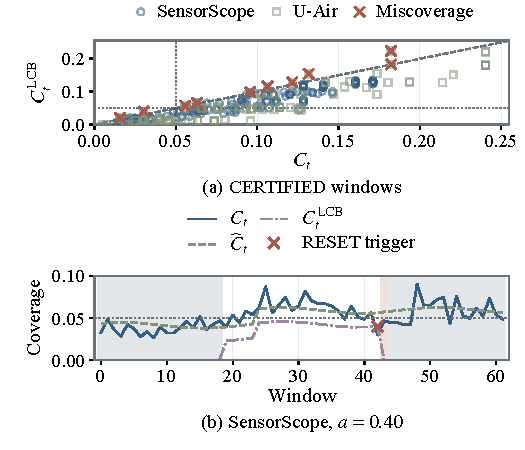
\includegraphics[width=\columnwidth]{fig_certificate_audit.pdf}
\caption{Coverage-controlled Design diagnostics.
(a)~CERTIFIED $C_t$ versus $C_t^{\mathrm{LCB}}$: crosses show miscoverage,
dashed $y=x$, dotted $\tau_{\mathrm{cov}}=0.05$.
(b)~SensorScope $a=0.40$: gray WARMUP, warm RESET; the cross triggers
next-window RESET. This Gate diagnostic is separate from configured Design.}
\label{fig:certificate_audit}
\end{figure}

\section{Development Learning and Implementation Sensitivity}
\AppNavLabel{app:development_details}
Independent development protocols retain their own targets and budgets.

\subsection{Centralized Learning Capacity and Baselines}
\AppNavLabel{app:learning_capacity}

Development seeds 41001--41003 use central-delivered training pools,
separate from main TEST. Both backbones run 200 effective passes, batch 64,
with Adam rates $.0003/.001/.003$ or momentum-SGD $.001/.01/.03$;
factor-.3 decay occurs at passes 50/100/150, and validation selects checkpoints.
HistoryResidual adds a 64/32 history network and training-statistic residual
to Common-NDMF. Counts are 108 central runs, one Traffic Uniform run and
three U-Air Central-all diagnostics. Figure~\ref{fig:learning_capacity} uses
Common-NDMF Adam $.003$ on Traffic/SensorScope, SGD $.03$ on U-Air;
HistoryResidual Adam $.003/.001/.003$, respectively.

\begin{table*}[t]
\centering
\caption{Central-delivered Common-NDMF validation against simple baselines.
Three development seeds; physical units. Gains are mean seed-paired relative
improvements over the strongest applicable simple baseline.}
\label{tab:learning_capacity}
\footnotesize
\begin{tabular*}{\textwidth}{@{\extracolsep{\fill}}llllrrr}
\toprule
Dataset & Unit & Optimizer / LR & Strongest simple baseline & Baseline RMSE & Model RMSE $\pm$ SD & Gain (\%)\\
\midrule
Traffic & vehicles/h & Adam / .003 & Weekly seasonal naive & 381.6185 & $202.0554\pm3.1556$ & $+47.01$\\
SensorScope & $^\circ$C & Adam / .003 & Training mean & 2.9687 & $2.6675\pm.0987$ & $+10.16$\\
U-Air & $\mu$g/m$^3$ & SGD / .03 & Spatial training mean & 20.3060 & $20.5015\pm.2311$ & $-0.96$\\
\bottomrule
\end{tabular*}
\end{table*}

\begin{figure*}[!tbp]
\centering
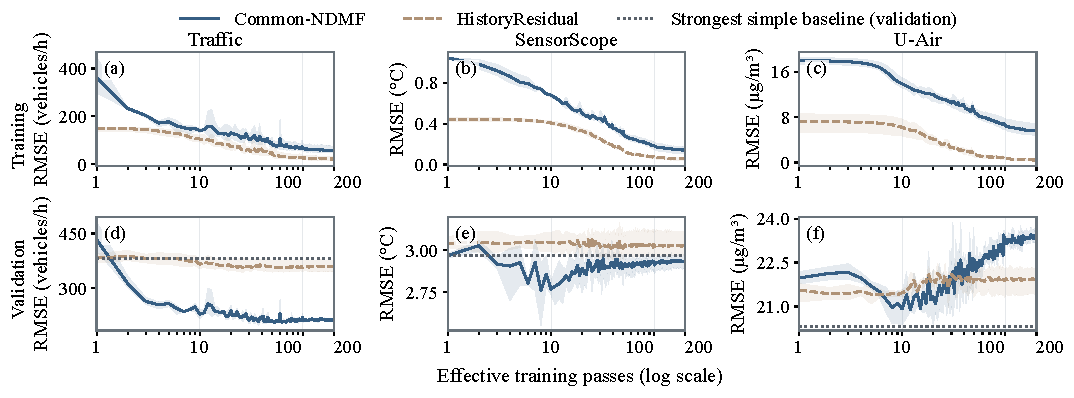
\includegraphics[width=\textwidth]{fig_learning_capacity_r2.pdf}
\caption{Centralized learning curves across datasets.
Central-delivered seeds 41001--41003; training/validation RMSE by row,
physical units by column. Lines/shading show means/seed min--max;
dotted validation baselines are seed means. The log axis counts effective
passes.}
\label{fig:learning_capacity}
\end{figure*}

Baselines use delivered training labels: means (training/spatial/seasonal),
persistence (latest legal observation) and seasonal naive (latest phase;
weekly needs two training weeks). Validation never enters history; scores
are inverse-scaled to float64 physical targets. HistoryResidual gains are
$7.33\%/-0.34\%/-4.45\%$ on Traffic/SensorScope/U-Air. U-Air Central-all
scores $19.5427$ versus spatial reference $18.4567$. Traffic Uniform reaches
$253.1132$ vehicles/h ($33.70\%$ improvement), improving $.914\%$ over passes 100--200.

\subsection{Formal-Protocol Prediction References}
\AppNavLabel{app:formal_prediction_references}

The training-mean predictors score $7.647/1.054/1.007$ on
SensorScope/U-Air/Traffic.  Constants fitted to the scored test labels score
$2.088/.678/1.007$ and are diagnostic references, not deployable baselines.
Training/test target means are $.301/7.657$, $0/-.807$, and $0/.003$,
respectively. Under the Complete-aligned station protocol, model RMSE on
both SensorScope and U-Air exceeds the corresponding training-mean baseline.

\subsection{Update-Rule Sensitivity}
\AppNavLabel{app:update_rule_sensitivity}

On NSW-Traffic (mean $K=12.1$, $15.1\%$ forced-Uniform active windows,
15 seeds), four federated rules including oracle margins agree within
$.002\%$ RMSE with the original server step. At 2/20 local steps, FedAvg
remains $2.8\%$--$3.0\%$ above centralized Adam ($10^{-3}$, 20 minibatches
of 32), with different optimizers and budgets; federated parameter movement is
$.26\%$--$.40\%$ of initial norm.

Server-only Adam ($\beta_1=.9$, $\beta_2=.99$, $\tau=10^{-3}$, rate $.003$,
one update/window) on 15 seeds unused for rate selection gives oracle-margin
RMSE headroom over FedAvg of $-1.49\%$ ($[-5.42,+1.76]\%$; 80\% MDE
$5.80\%$), without establishing $.5\%$ equivalence. Mean RMSE is
$.967/.973$, ranges $[.659,1.572]/[.795,1.459]$, versus the $1.007$ constant
reference. Oracle weights reduce group/client--stratum mismatch by
$.0079$ ($[.0051,.0110]$) and $.0099$ ($[.0067,.0132]$) on these runs.

\subsection{Development Constraint Geometry}
\AppNavLabel{app:development_geometry}

Table~\ref{tab:development_geometry} reports natural-window geometry;
Table~\ref{tab:geometry_sensitivity} varies caps and ESS on fixed-client subsets.
Initial development updates retain their correction settings. Windows
with at least eight clients use the first eight in sorted order and a
renormalized reference. Feasible ranges separate weight freedom from mass
adjustable by at least .01, without prediction re-evaluation.

\begin{table}[!htbp]
\centering
\caption{Natural-window geometry under the separate development protocol.
Seeds 41001--41003, cap .5, ESS minimum 3.}
\label{tab:development_geometry}
\footnotesize
\setlength{\tabcolsep}{3pt}
\begin{tabular}{lrrrr}
\toprule
Dataset & Windows & $K$ range & Singleton (\%) & Adj. mass (\%)\\
\midrule
SensorScope & 283 & 1--6 & 80.57 & 0.433\\
U-Air & 228 & 1--6 & 82.46 & 0.515\\
Traffic & 300 & 1--15 & 4.33 & 4.647\\
\bottomrule
\end{tabular}
\end{table}

\begin{table}[!htbp]
\centering
\caption{NSW-Traffic geometry under cap and ESS changes.
183 fixed-$K=8$ subsets. $E$: minimum ESS; cap: maximum weight;
repair: mean $\|\operatorname{Proj}_{\mathcal C}(\widehat\beta)-\widehat\beta\|_2$.
Adjustable mass remains $4.651\%$.}
\label{tab:geometry_sensitivity}
\footnotesize
\setlength{\tabcolsep}{4pt}
\begin{tabular*}{\columnwidth}{@{\extracolsep{\fill}}rrrr}
\toprule
$E$ & Cap & Reference violates (\%) & Repair\\
\midrule
2.0 & .2500 & 59.02 & .067487\\
4.0 & .2500 & 59.02 & .067487\\
6.4 & .2500 & 68.85 & .074626\\
4.0 & .1875 & 96.17 & .126015\\
4.0 & .5000 & 12.02 & .010304\\
\bottomrule
\end{tabular*}
\end{table}

No natural payload has $K=16$; tighter caps increase infeasibility/projection
distance, not .01-threshold adjustable mass. No forecasts or label-dependent
choices enter this diagnostic.

